%---------------
% LIBVIRT INSTALL
%---------------

\section{libvirt 0.8.7 installation}
\label{app:libvirt}
POP-C++ Virtual Secure uses libvirt to interact with the ESXi platform. We need to install libvirt before compiling and installing POP-C++. \s

The latest version of libvirt is available at : http://www.libvirt.org\s

To install libvirt, we need first to install some packages. On a Debian/Ubuntu Os we can use apt-get to install the following packages: \s

\begin{lstlisting}
sudo apt-get install libxml2 libxml2-dev libgnutls-dev libdevmapper-dev 
libcurl4-openssl-dev libvirt-dev libnl-dev
\end{lstlisting}\s

After the installation of these packages, we need to install the libvirt distribution downloaded from the official libvirt website. To configure libvirt with the ESXi driver use the following command: \s

\begin{lstlisting}
./configure --with-esx=yes
\end{lstlisting}\s

We can make sure that the ESX driver support is enabled by checking the end of the configure script output. We should have the following line:\s

\begin{lstlisting}
configure: ESX: yes
\end{lstlisting}\s

Once the configure process is done, we can compile and install libvirt. Use the following commands to do that. \s

\begin{lstlisting}
make 
sudo make install
\end{lstlisting}



%---------------
% VMWARE TOOLS INSTALL
%---------------
\pagebreak
\section{VMware Tools 8.3.2 installation}
\label{app:vmwaretools}
To install the latest VMware tools on the VM, we need to use the vSphere Client. On the left side, we need to right-click on the VM and select Guest > Install/Upgarde VMware Tools (see Figure \ref{fig:vmwaretoolsinstall1}). This action will connect a virtual CD-ROM on the VM. 

\begin{figure}[ht]
	\caption{VMware Tools Install (Step 1) }
  	\centering
	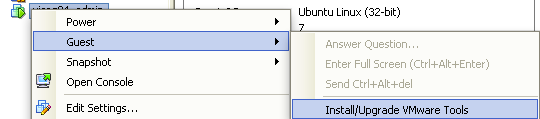
\includegraphics[width=0.5\textwidth]{./pic/vmwaretools_1.png}
	\label{fig:vmwaretoolsinstall1}
\end{figure}

Once the CD-ROM is connected to the VM, we need to mount it. Use the following command to mount it and to launch the installation process. We do a default installation. \s

\begin{lstlisting}
sudo mount /dev/cdrom /media/cdrom
cp /media/cdrom/VMwareTools-8.3.2-257589.tar.gz ./
tar -xvf VMwareTools-8.3.2-257589.tar.gz
cd vmware-tools-distrib
sudo ./vmware-install.pl
\end{lstlisting}




%---------------
% VMWARE CLI INSTALL
%---------------

\section{VMware CLI 4.1 installation}
\label{app:vmwarecli}

The VMware CLI are used by POP-C++ to do some action that are not currently possible with libvirt such as the cloning process. \s

The latest version of the VMware CLI can be found at : http://www.vmware.com/support/developer/vcli/ \s

To install the VMware CLI, we need first to install some packages. On a Debian/Ubuntu Os we can use apt-get to install the following packages: \s

\begin{lstlisting}
sudo apt-get install libcrypt-ssleay-perl libssl-dev libxml-libxml-perl
\end{lstlisting}

After the installation of these packages, we can install the VMware CLI itself. To do it, use the following commands:\s

\begin{lstlisting}
tar -xvf VMware-vSphere-CLI-4.1.0-254719.i386.tar.gz
cd vmware-vsphere-cli-distrib
sudo ./vmware-install.pl
\end{lstlisting}\s

Just follow the installation script and enter default values. 




%---------------
% VIX INSTALL
%---------------
\pagebreak
\section{VIX 1.10.2 installation}
\label{app:vix}
The VMware VIX API is used by POP-C++ for some action that are not currently available in libvirt such as sending file to a VM or executing command on VM.\s

The latest version of VIX can be found at : http://www.vmware.com/support/developer/vix-api/

To install the VIX API, we just run the bundle with the following command: \s

\begin{lstlisting}
sudo sh VMware-VIX-1.10.2-331863.i386.bundle
\end{lstlisting}



%---------------
% ESXI INSTALL
%---------------
\section{VMware ESXi 4.1}
\label{app:esxi}
The first step is to install the ESXi hypervisor on your hardware if it's not done already. Be sure that your hardware is listed in the "Hardware Compatibility Guide" (http://www.vmware.com/resources/compatibility/search.php). \s

The latest version of VMware ESXi can be found at: http://www.vmware.com/products/vsphere-hypervisor/

\textbf{Step 1:}\\
We first need a bootable CD-ROM of ESXi 4.1 or later. Once the CD-ROM is in the computer and the computer is started, the "VWware ESXi Boot Menu" will appear. At this step, we need to choose to boot from the ESXi Installer. 

\begin{figure}[ht]
	\caption{VMware ESXi Boot Menu}
  	\centering
	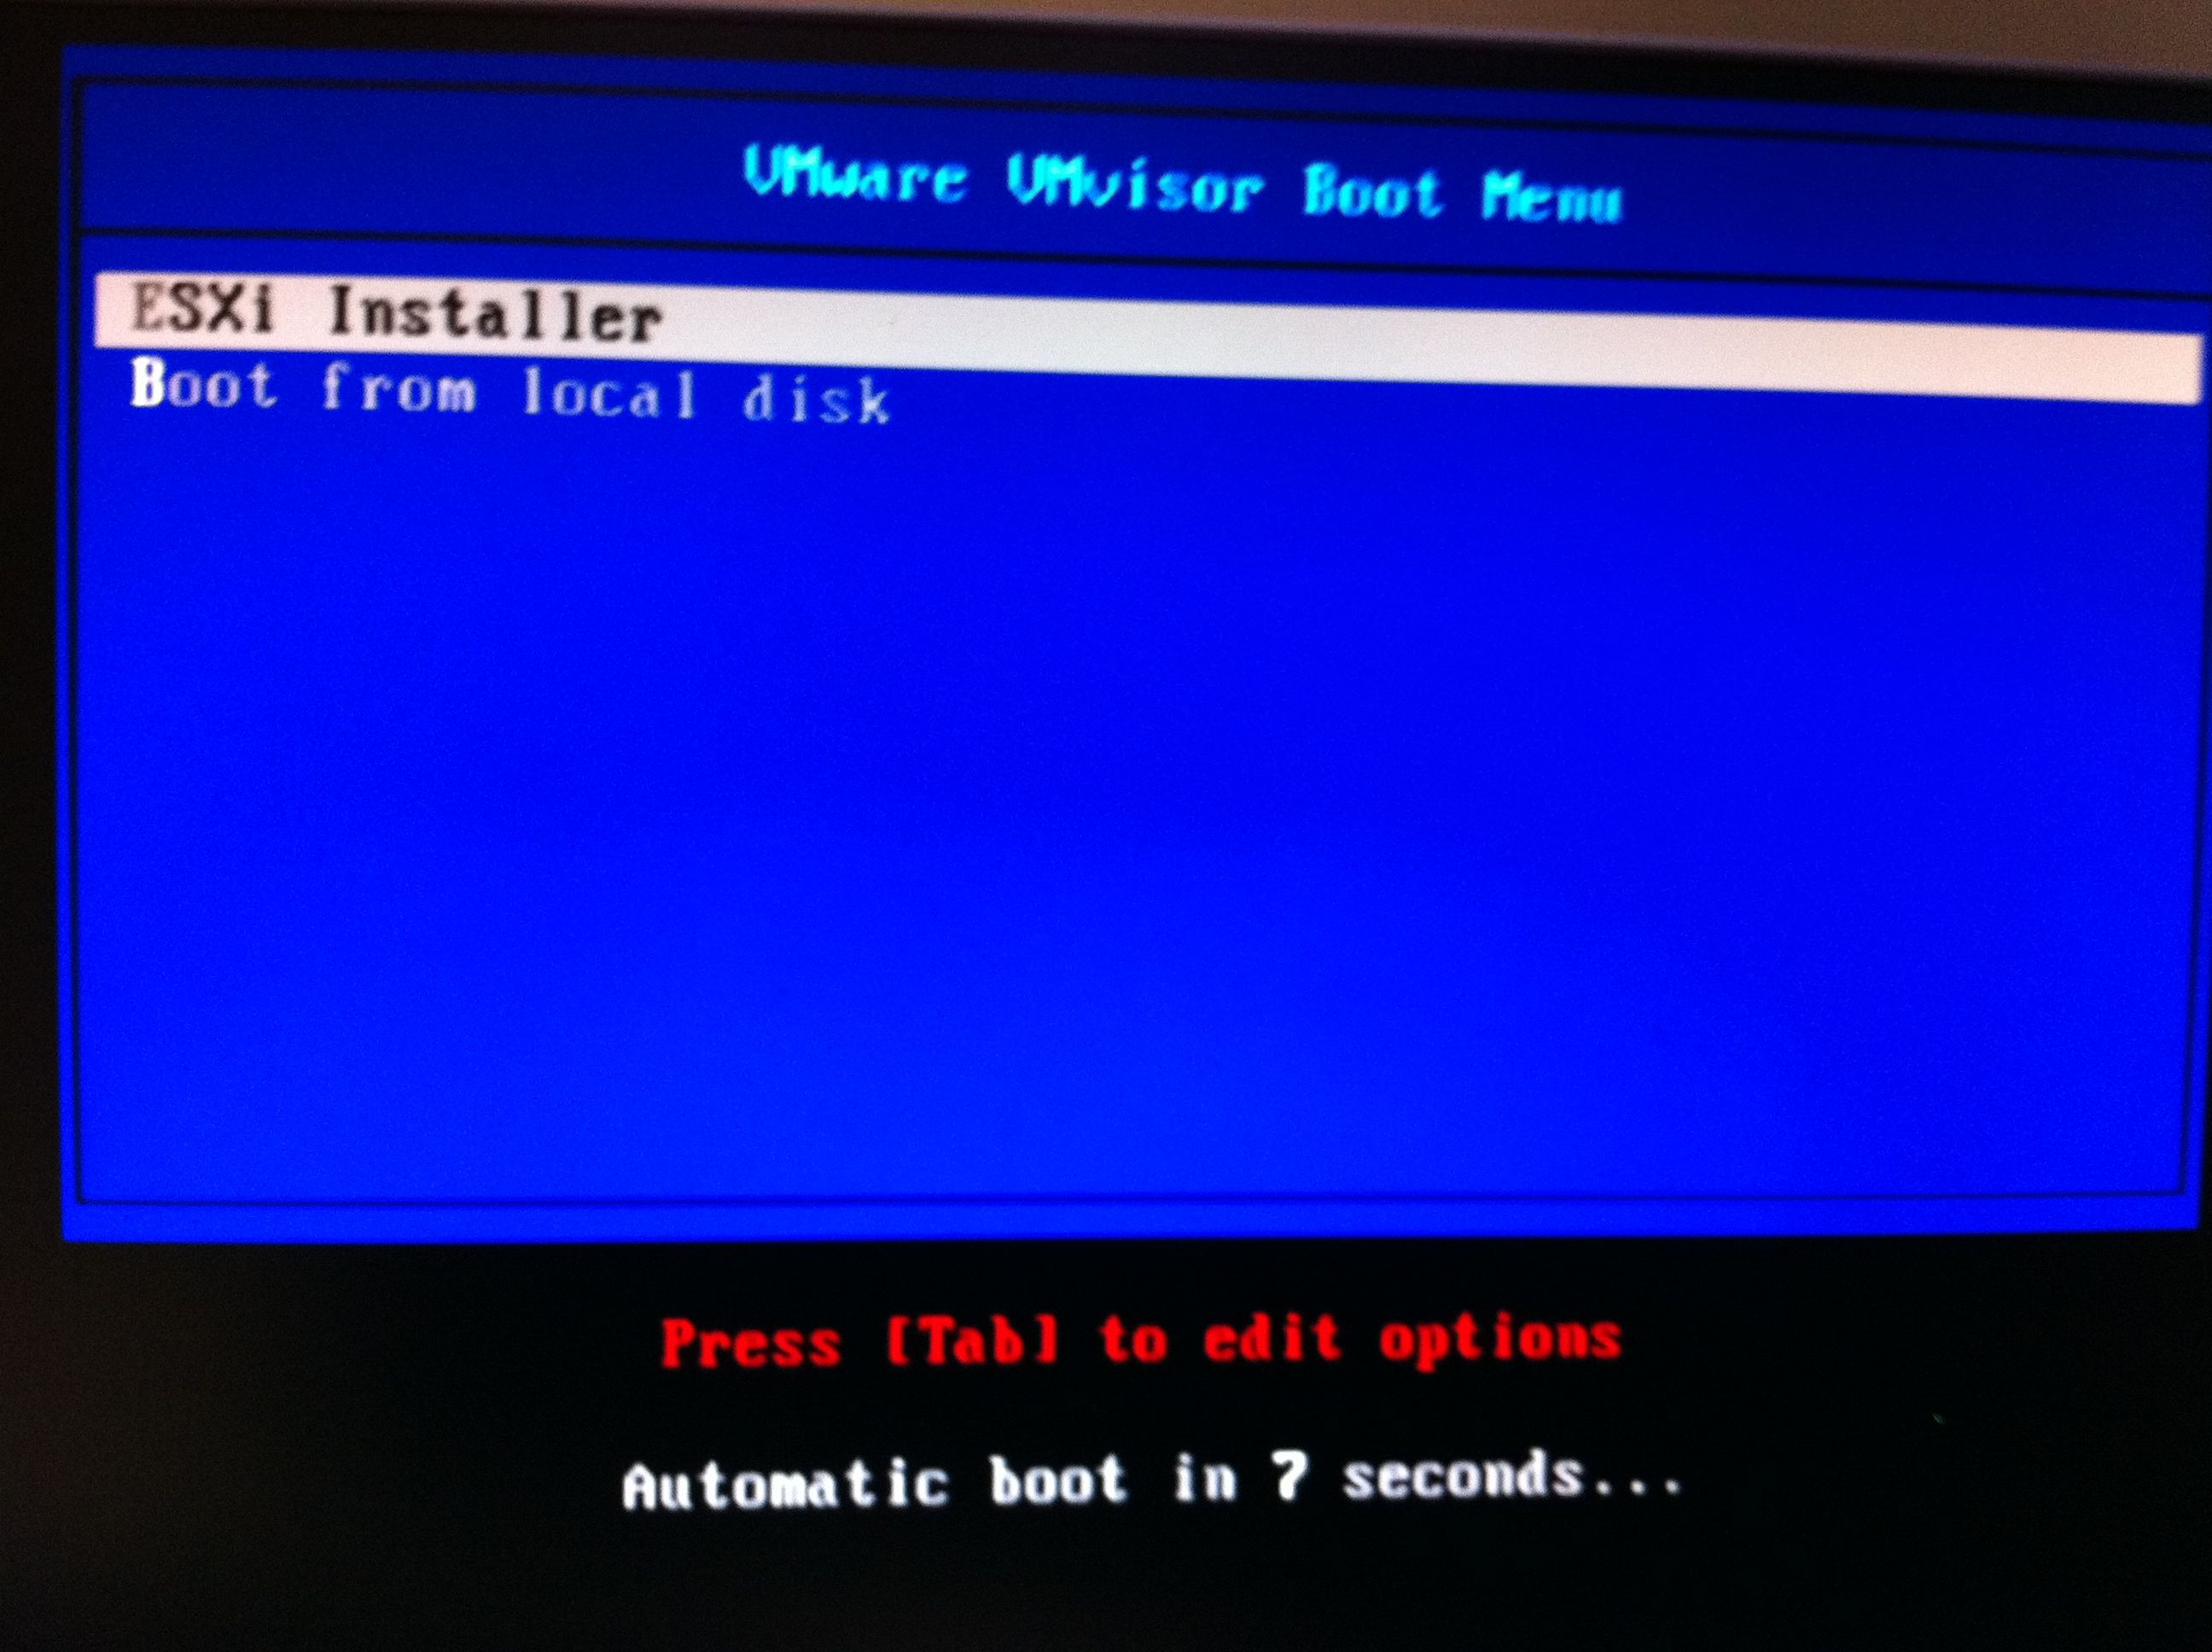
\includegraphics[width=0.5\textwidth]{./pic/esxi_1.jpg}
	\label{fig:kex_object_creation}
\end{figure}

\textbf{Step 2:}\\
Once the installer has started, the welcome screen will be displayed. On this screen, we would choose the "Install" option by pressing the "Enter" key. 

\begin{figure}[ht]
	\caption{VMware ESXi Installation Welcome screen}
  	\centering
	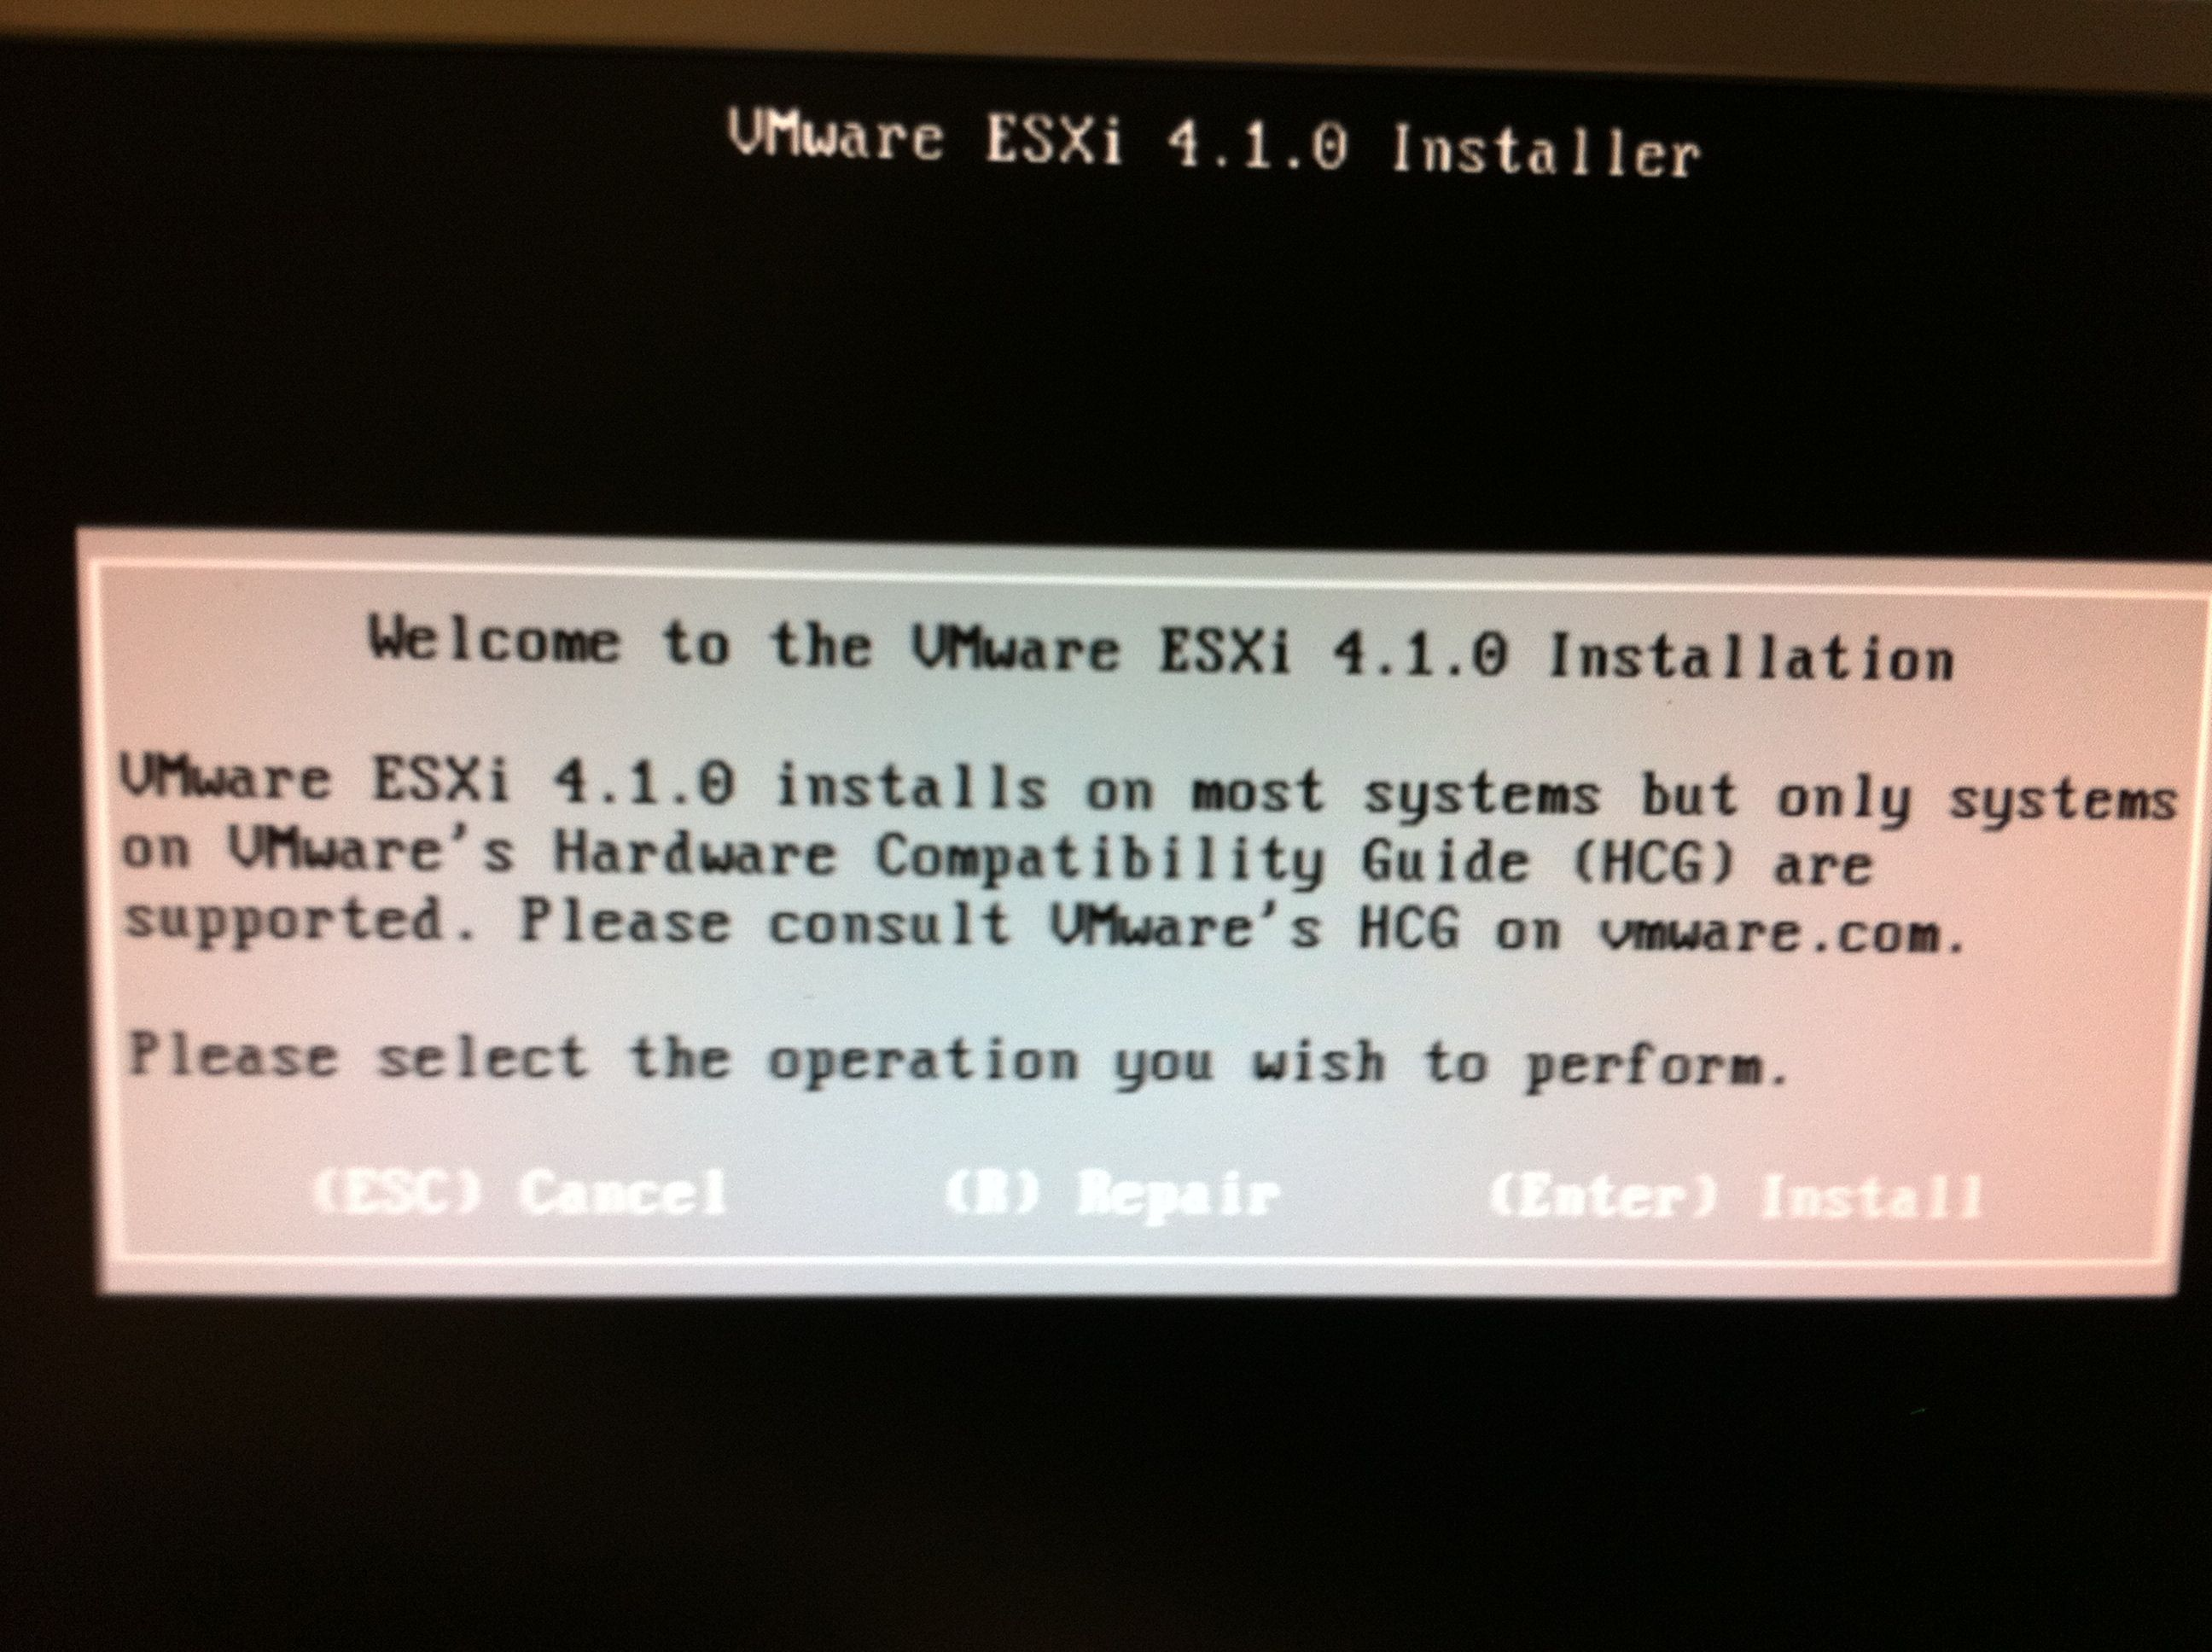
\includegraphics[width=0.5\textwidth]{./pic/esxi_2.jpg}
	\label{fig:kex_object_creation}
\end{figure}

\pagebreak
\textbf{Step 3:}\\
We will need to agree the licence of VMware ESXi by pressing the "F11" key. 
\begin{figure}[ht]
	\caption{VMware ESXi licence agreement}
  	\centering
	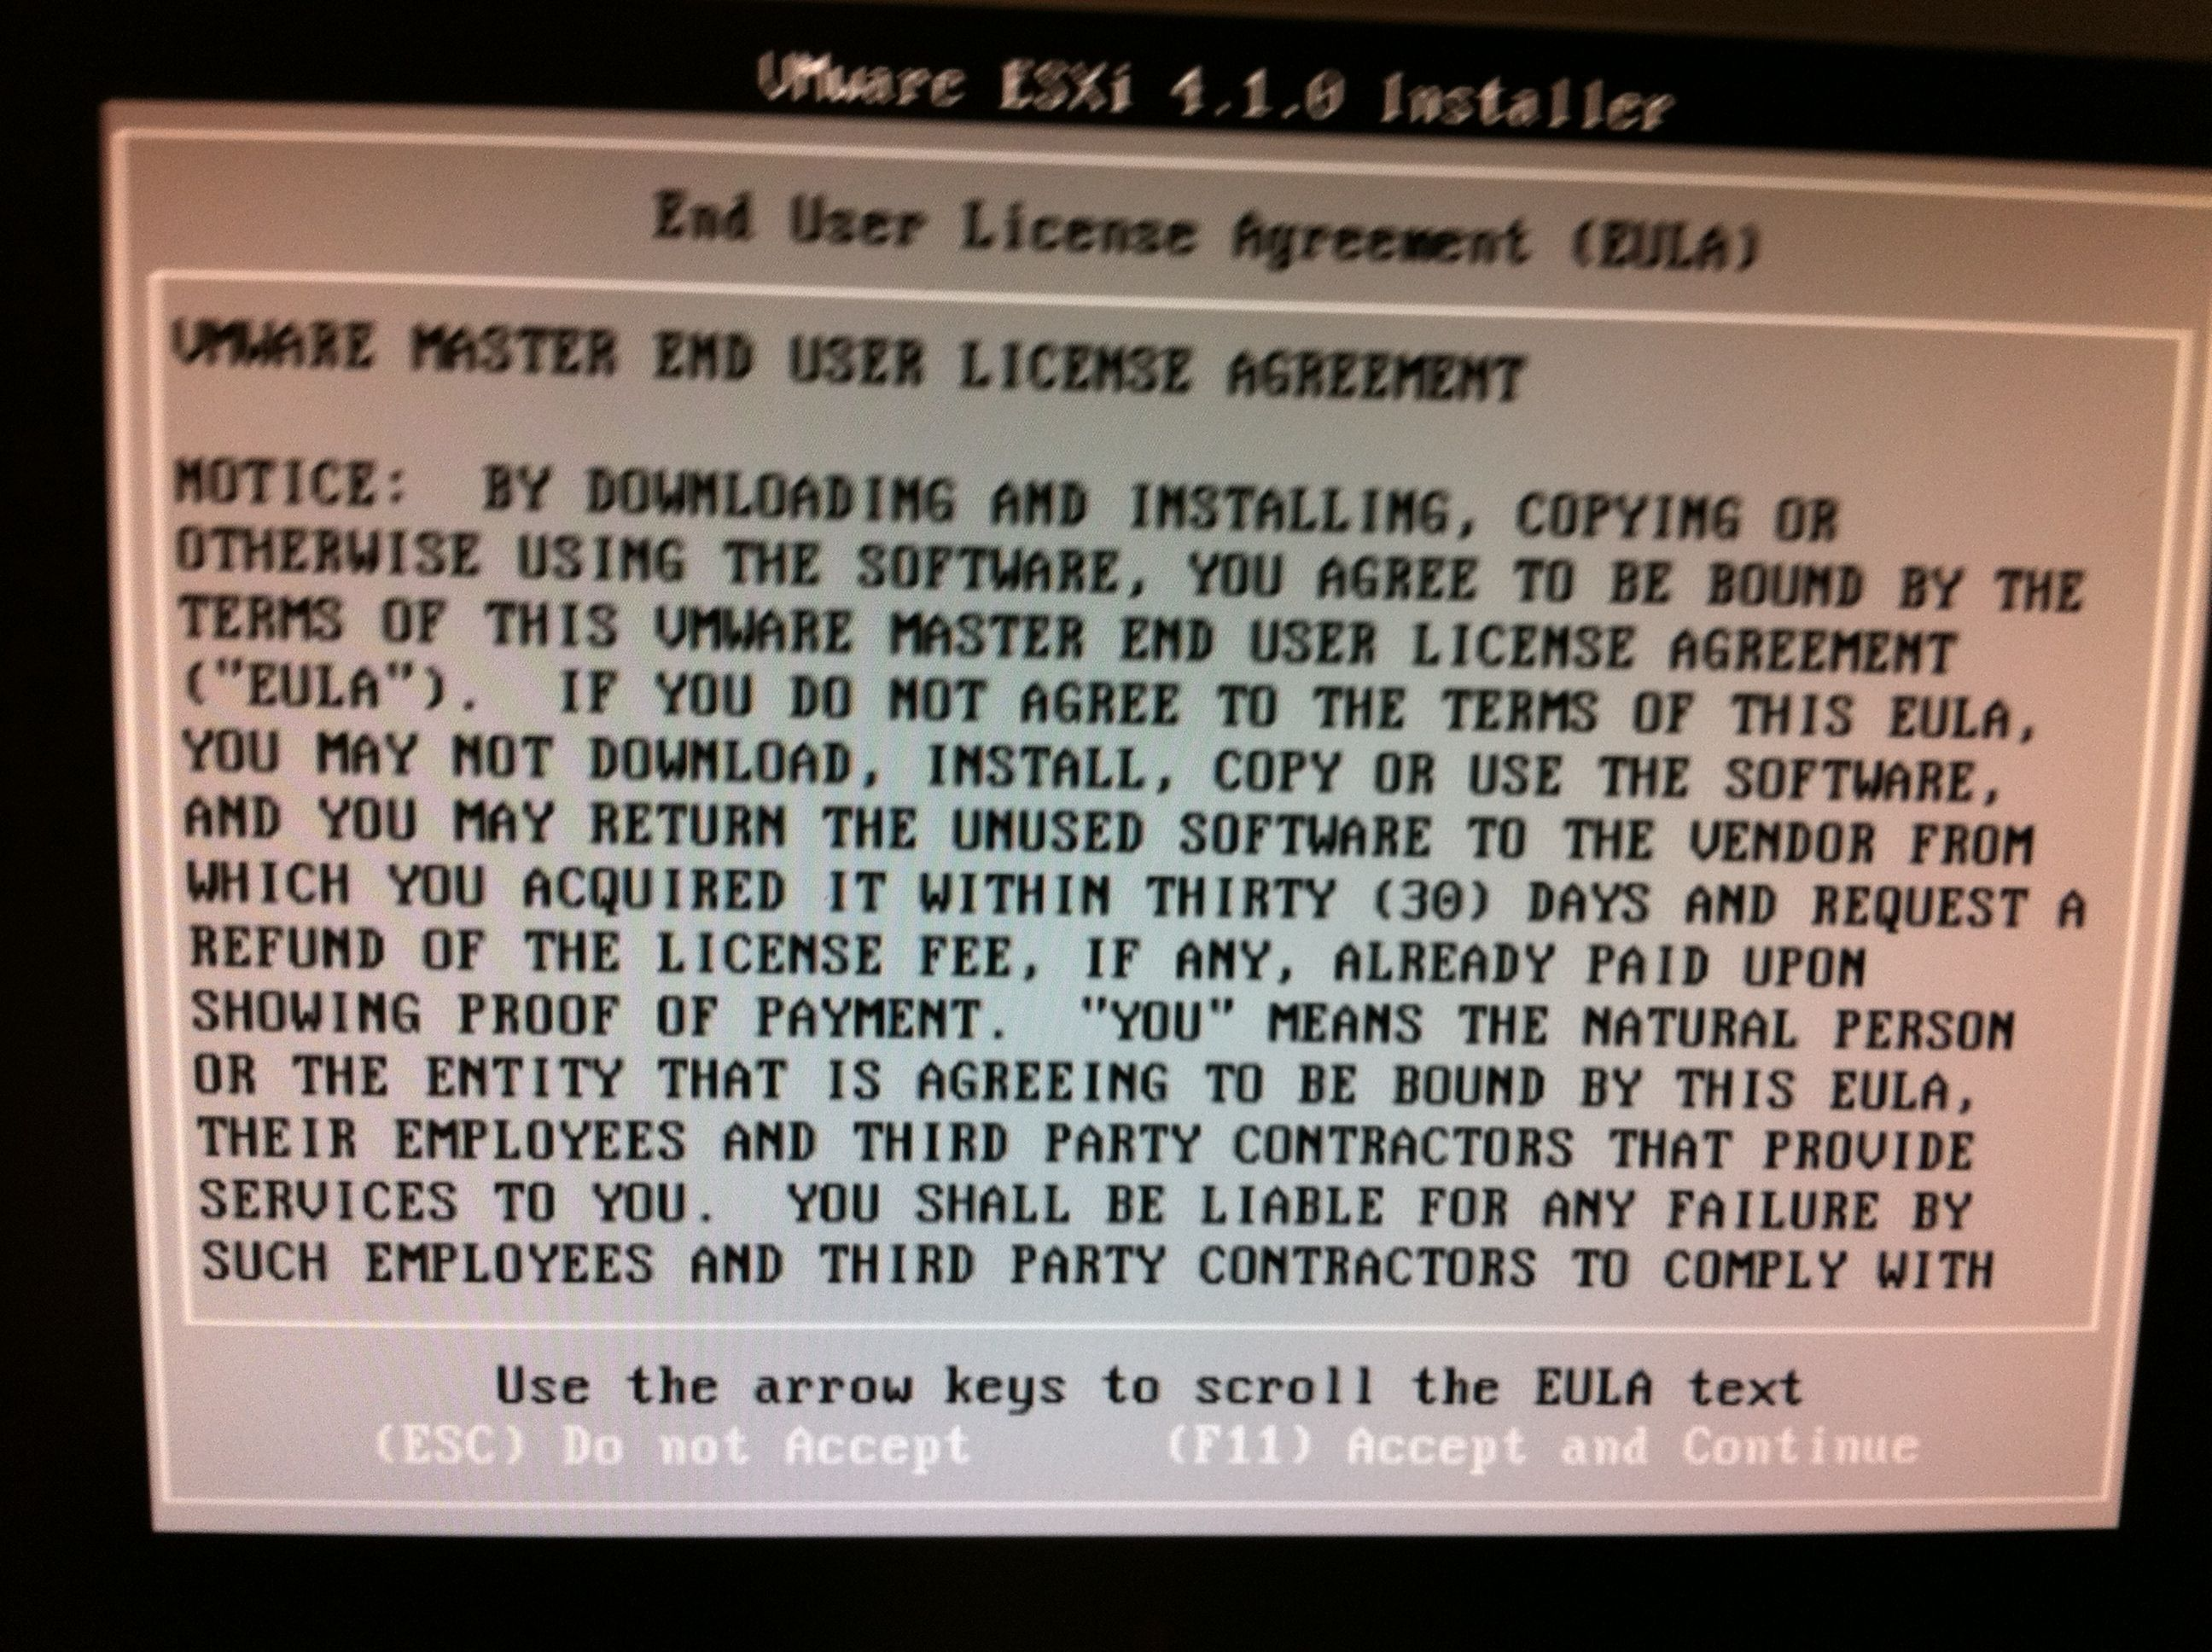
\includegraphics[width=0.5\textwidth]{./pic/esxi_3.jpg}
	\label{fig:kex_object_creation}
\end{figure}

\textbf{Step 4:}\\
In this step, we will need to choose the disk to install VMware ESXi. We choose the correct destination disk and press "Enter"
\begin{figure}[ht]
	\caption{VMware ESXi disk selection}
  	\centering
	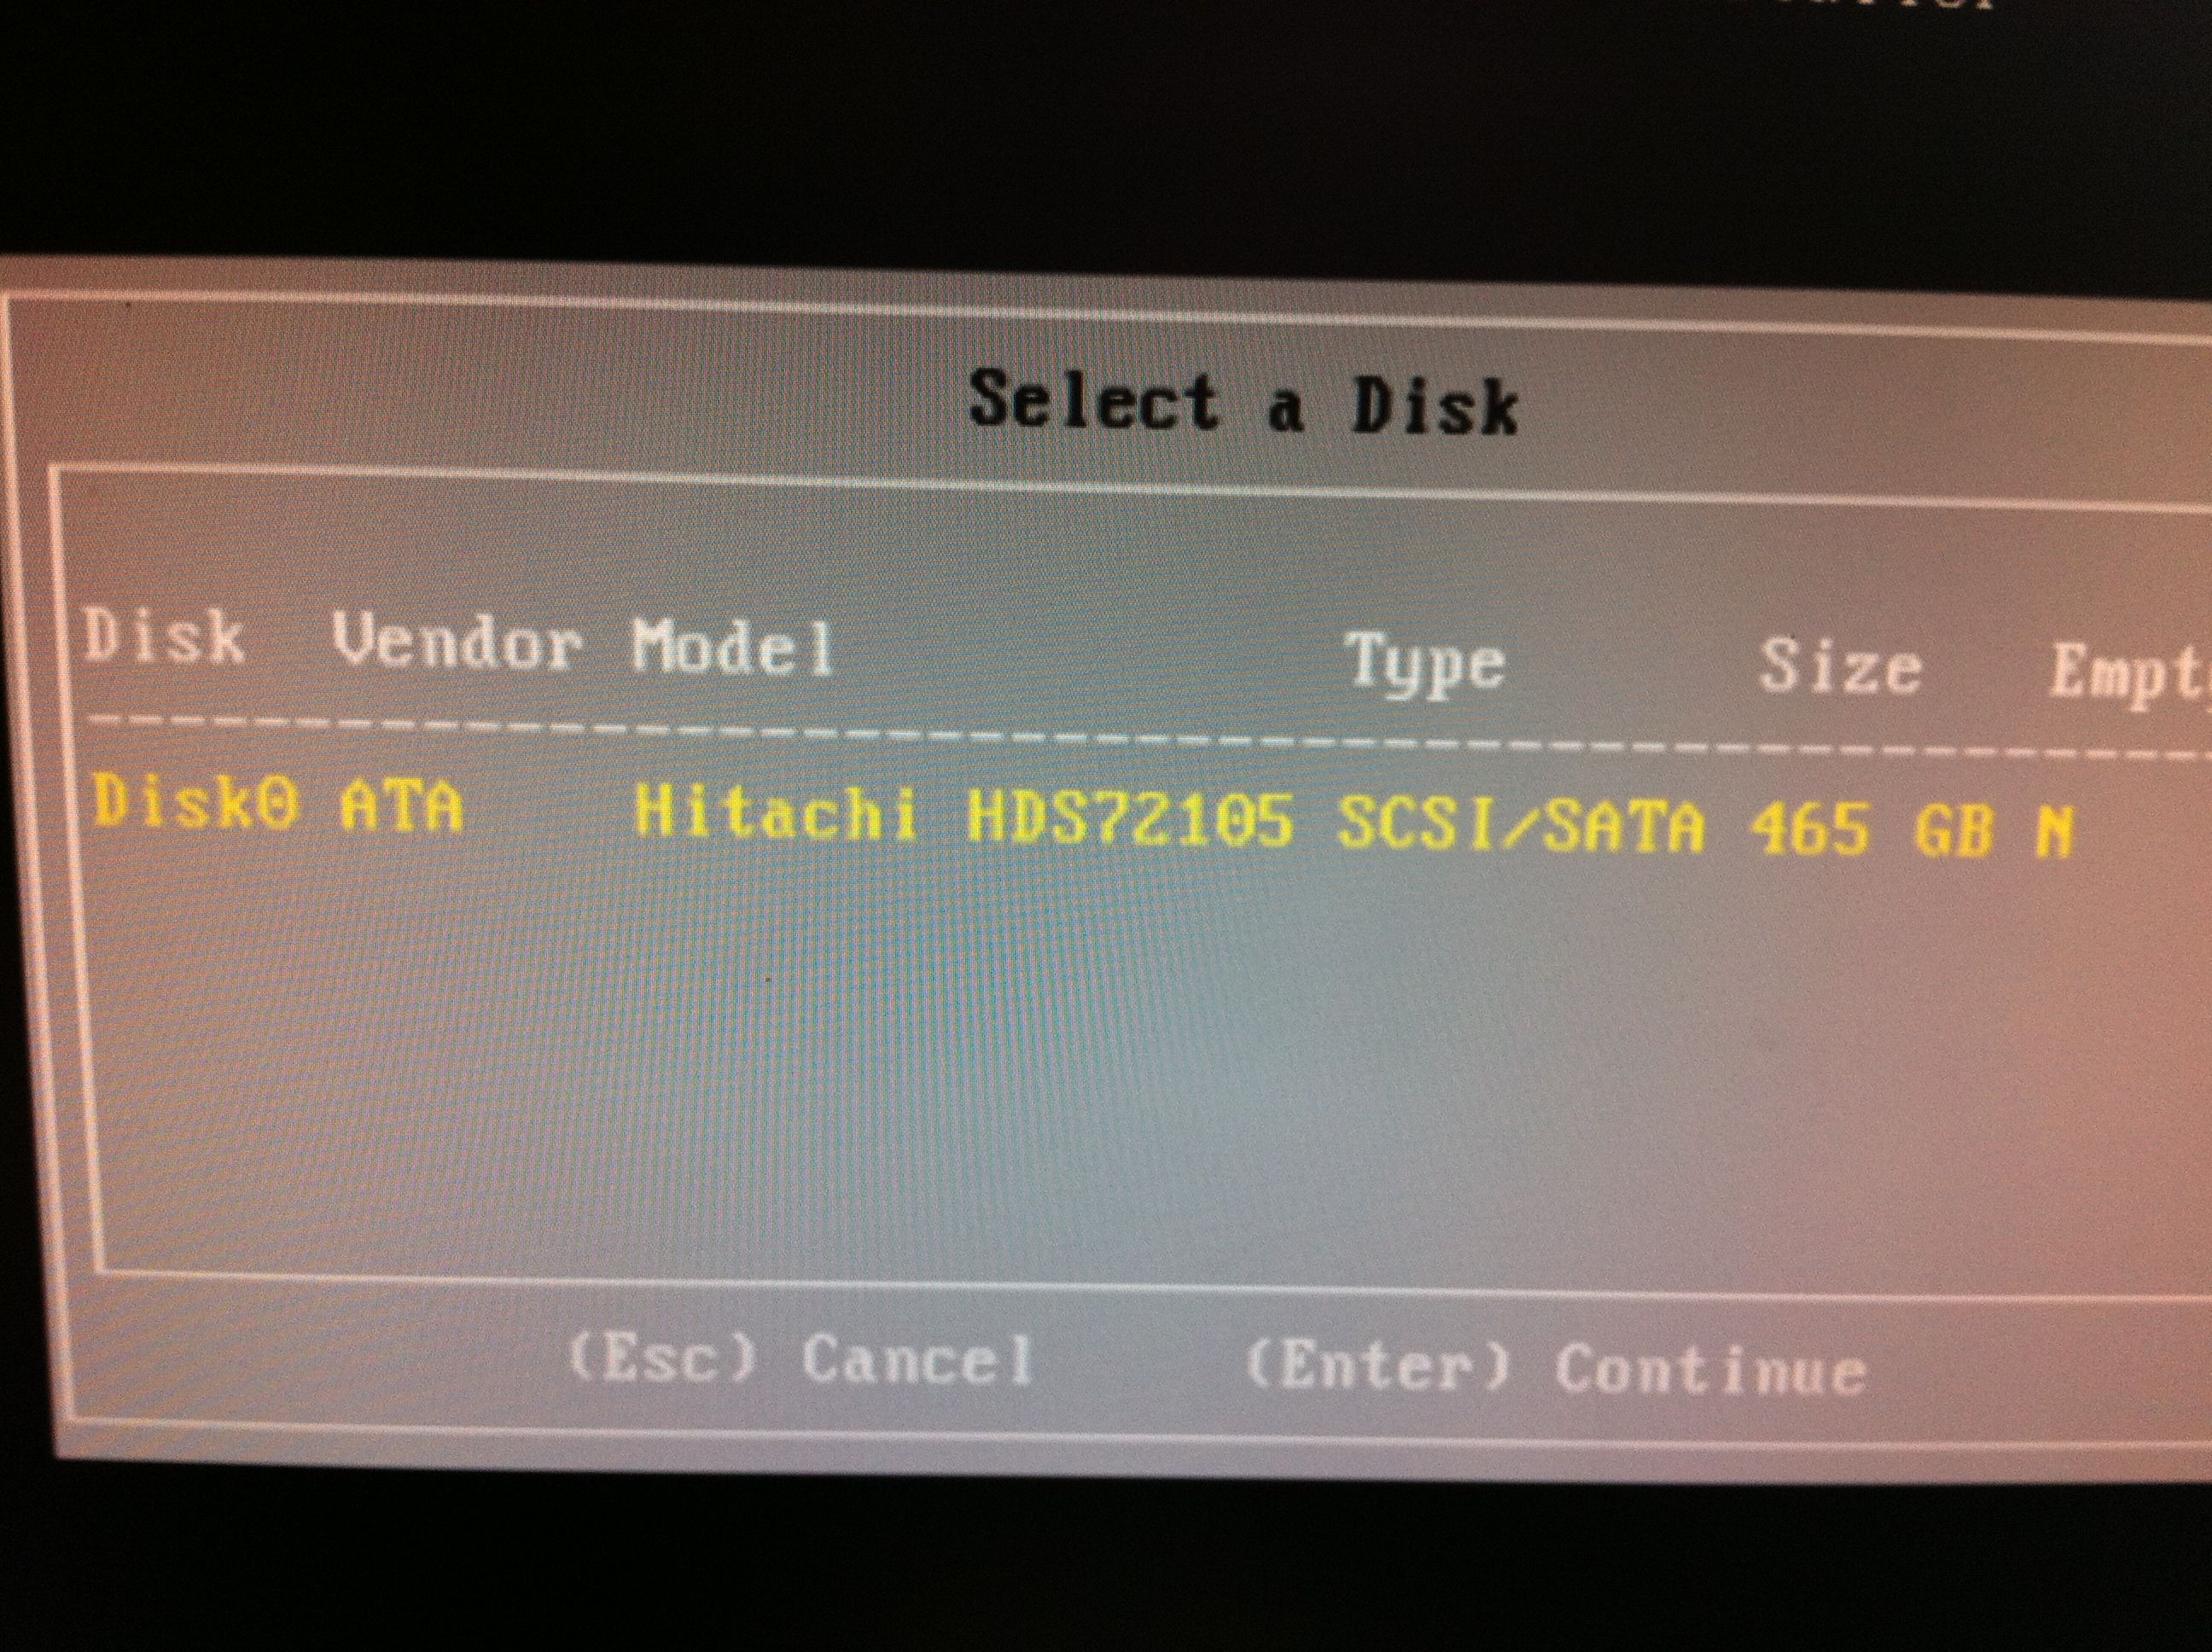
\includegraphics[width=0.5\textwidth]{./pic/esxi_4.jpg}
	\label{fig:kex_object_creation}
\end{figure}

\pagebreak
\textbf{Step 5: (optional)}\\
The installation program may ask if we want to erase the data containing on the destination disk. We will erase the data by pressing the "Enter" key. 
\begin{figure}[ht]
	\caption{VMware ESXi disk selection (confirmation)}
  	\centering
	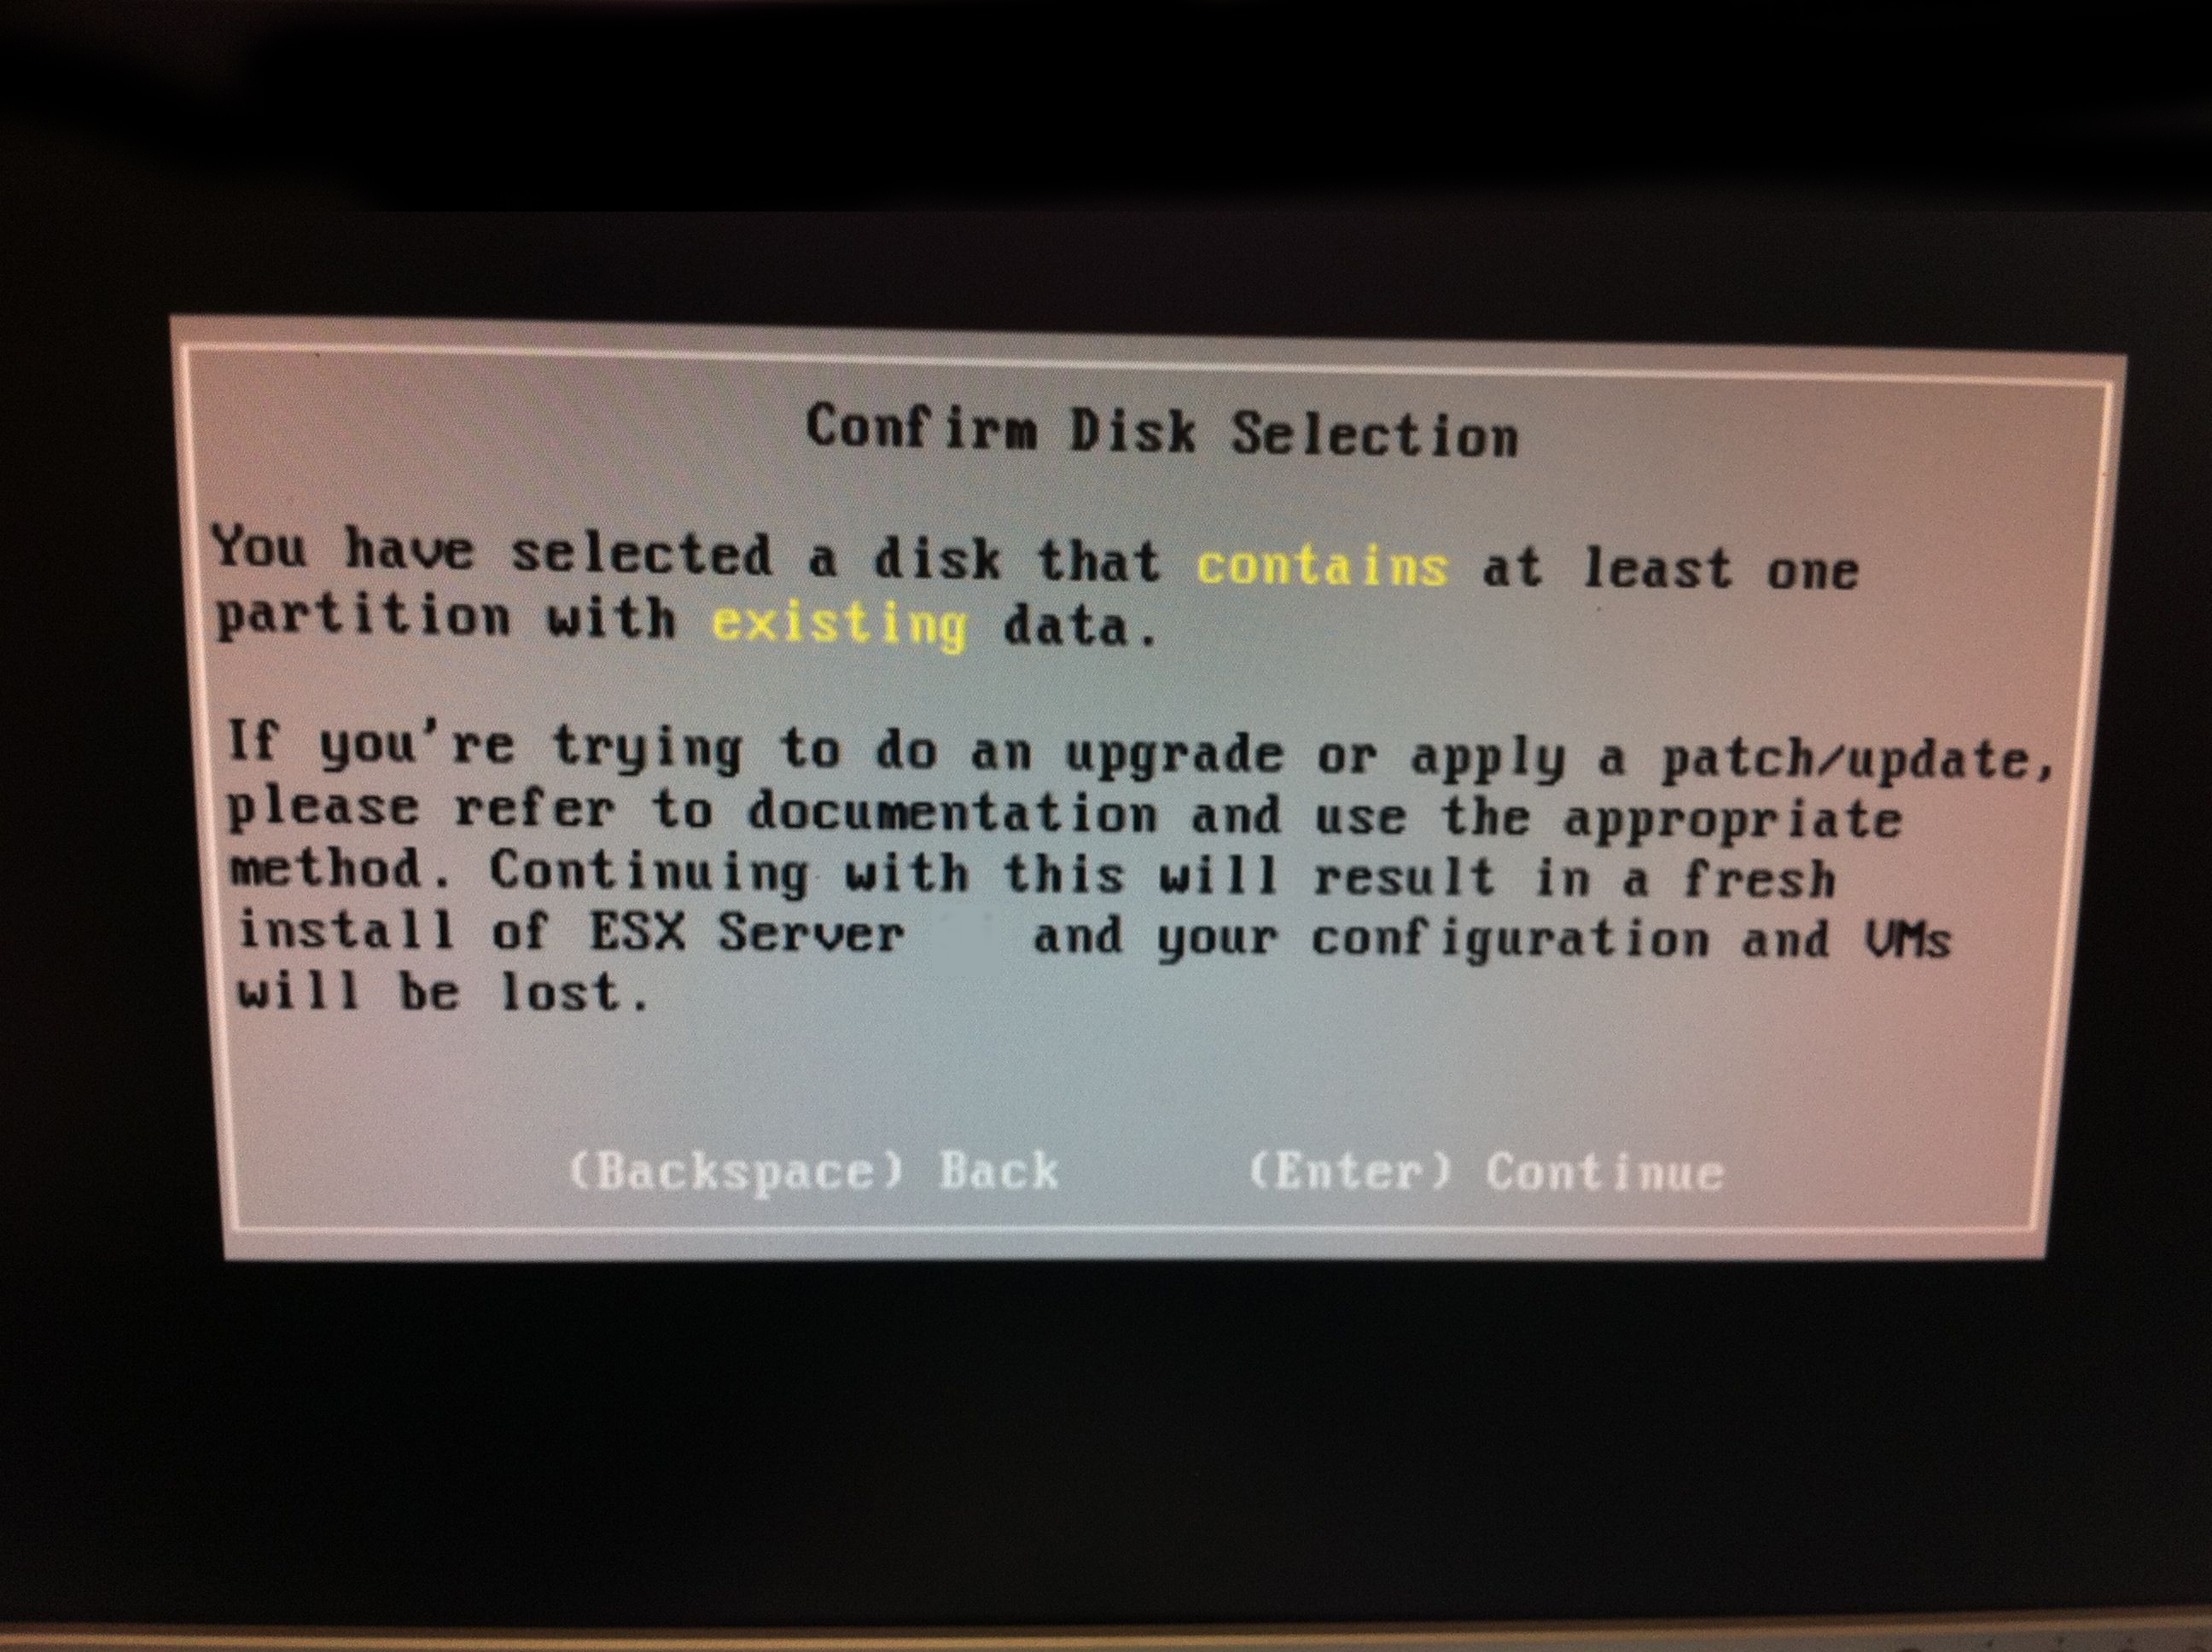
\includegraphics[width=0.5\textwidth]{./pic/esxi_5.jpg}
	\label{fig:kex_object_creation}
\end{figure}

\textbf{Step 6:}\\
We are ready to launch the installation of VMware ESXi on the computer. The installation program will ask us to confirm the installation by pressing the "F11" key. 
\begin{figure}[ht]
	\caption{VMware ESXi Installation confirmation}
  	\centering
	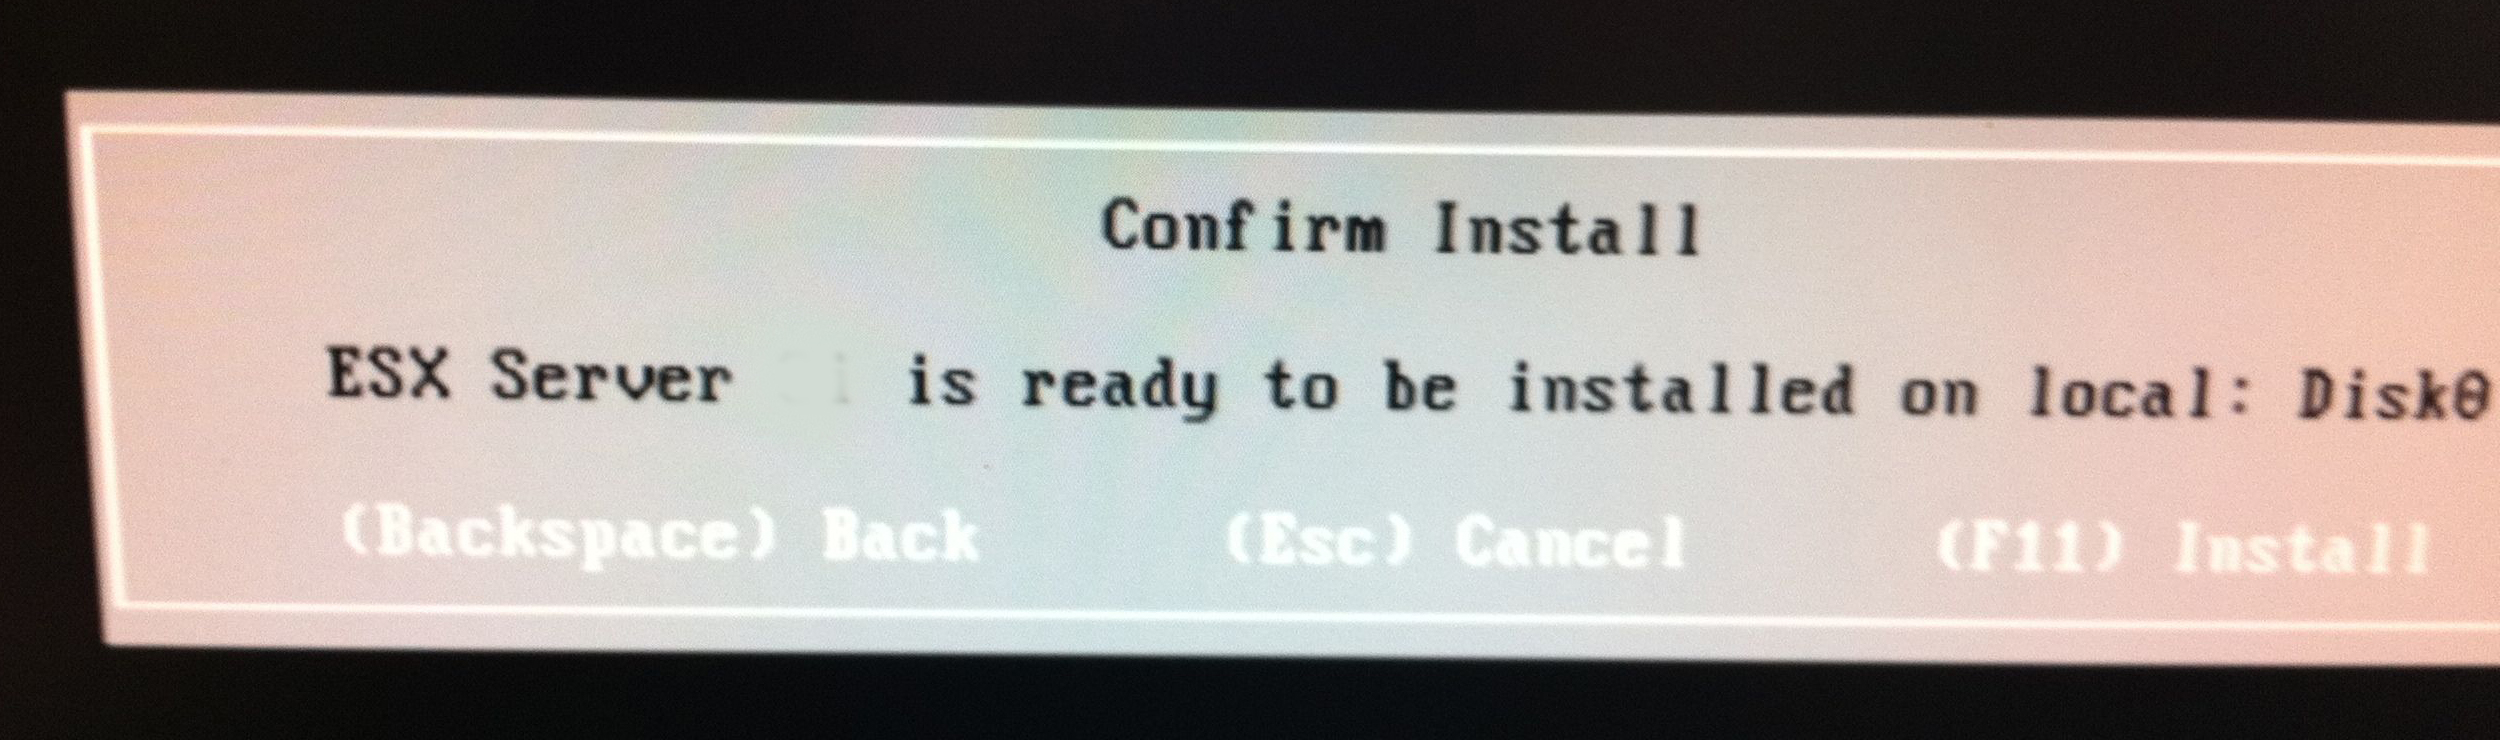
\includegraphics[width=0.7\textwidth]{./pic/esxi_6.jpg}
	\label{fig:kex_object_creation}
\end{figure}


\pagebreak
\textbf{ESXi configuration}
As the ESXi platform will act as a server, we will need to configure the network parameter and the credentials. When the ESXi system is started, the first screen looks like Firgure \ref{fig:esxi_first_screen}. To be able to change any system parameters, we need to press the "F2" key.\s

\begin{figure}[ht]
	\caption{VMware ESXi Startup screen}
  	\centering
	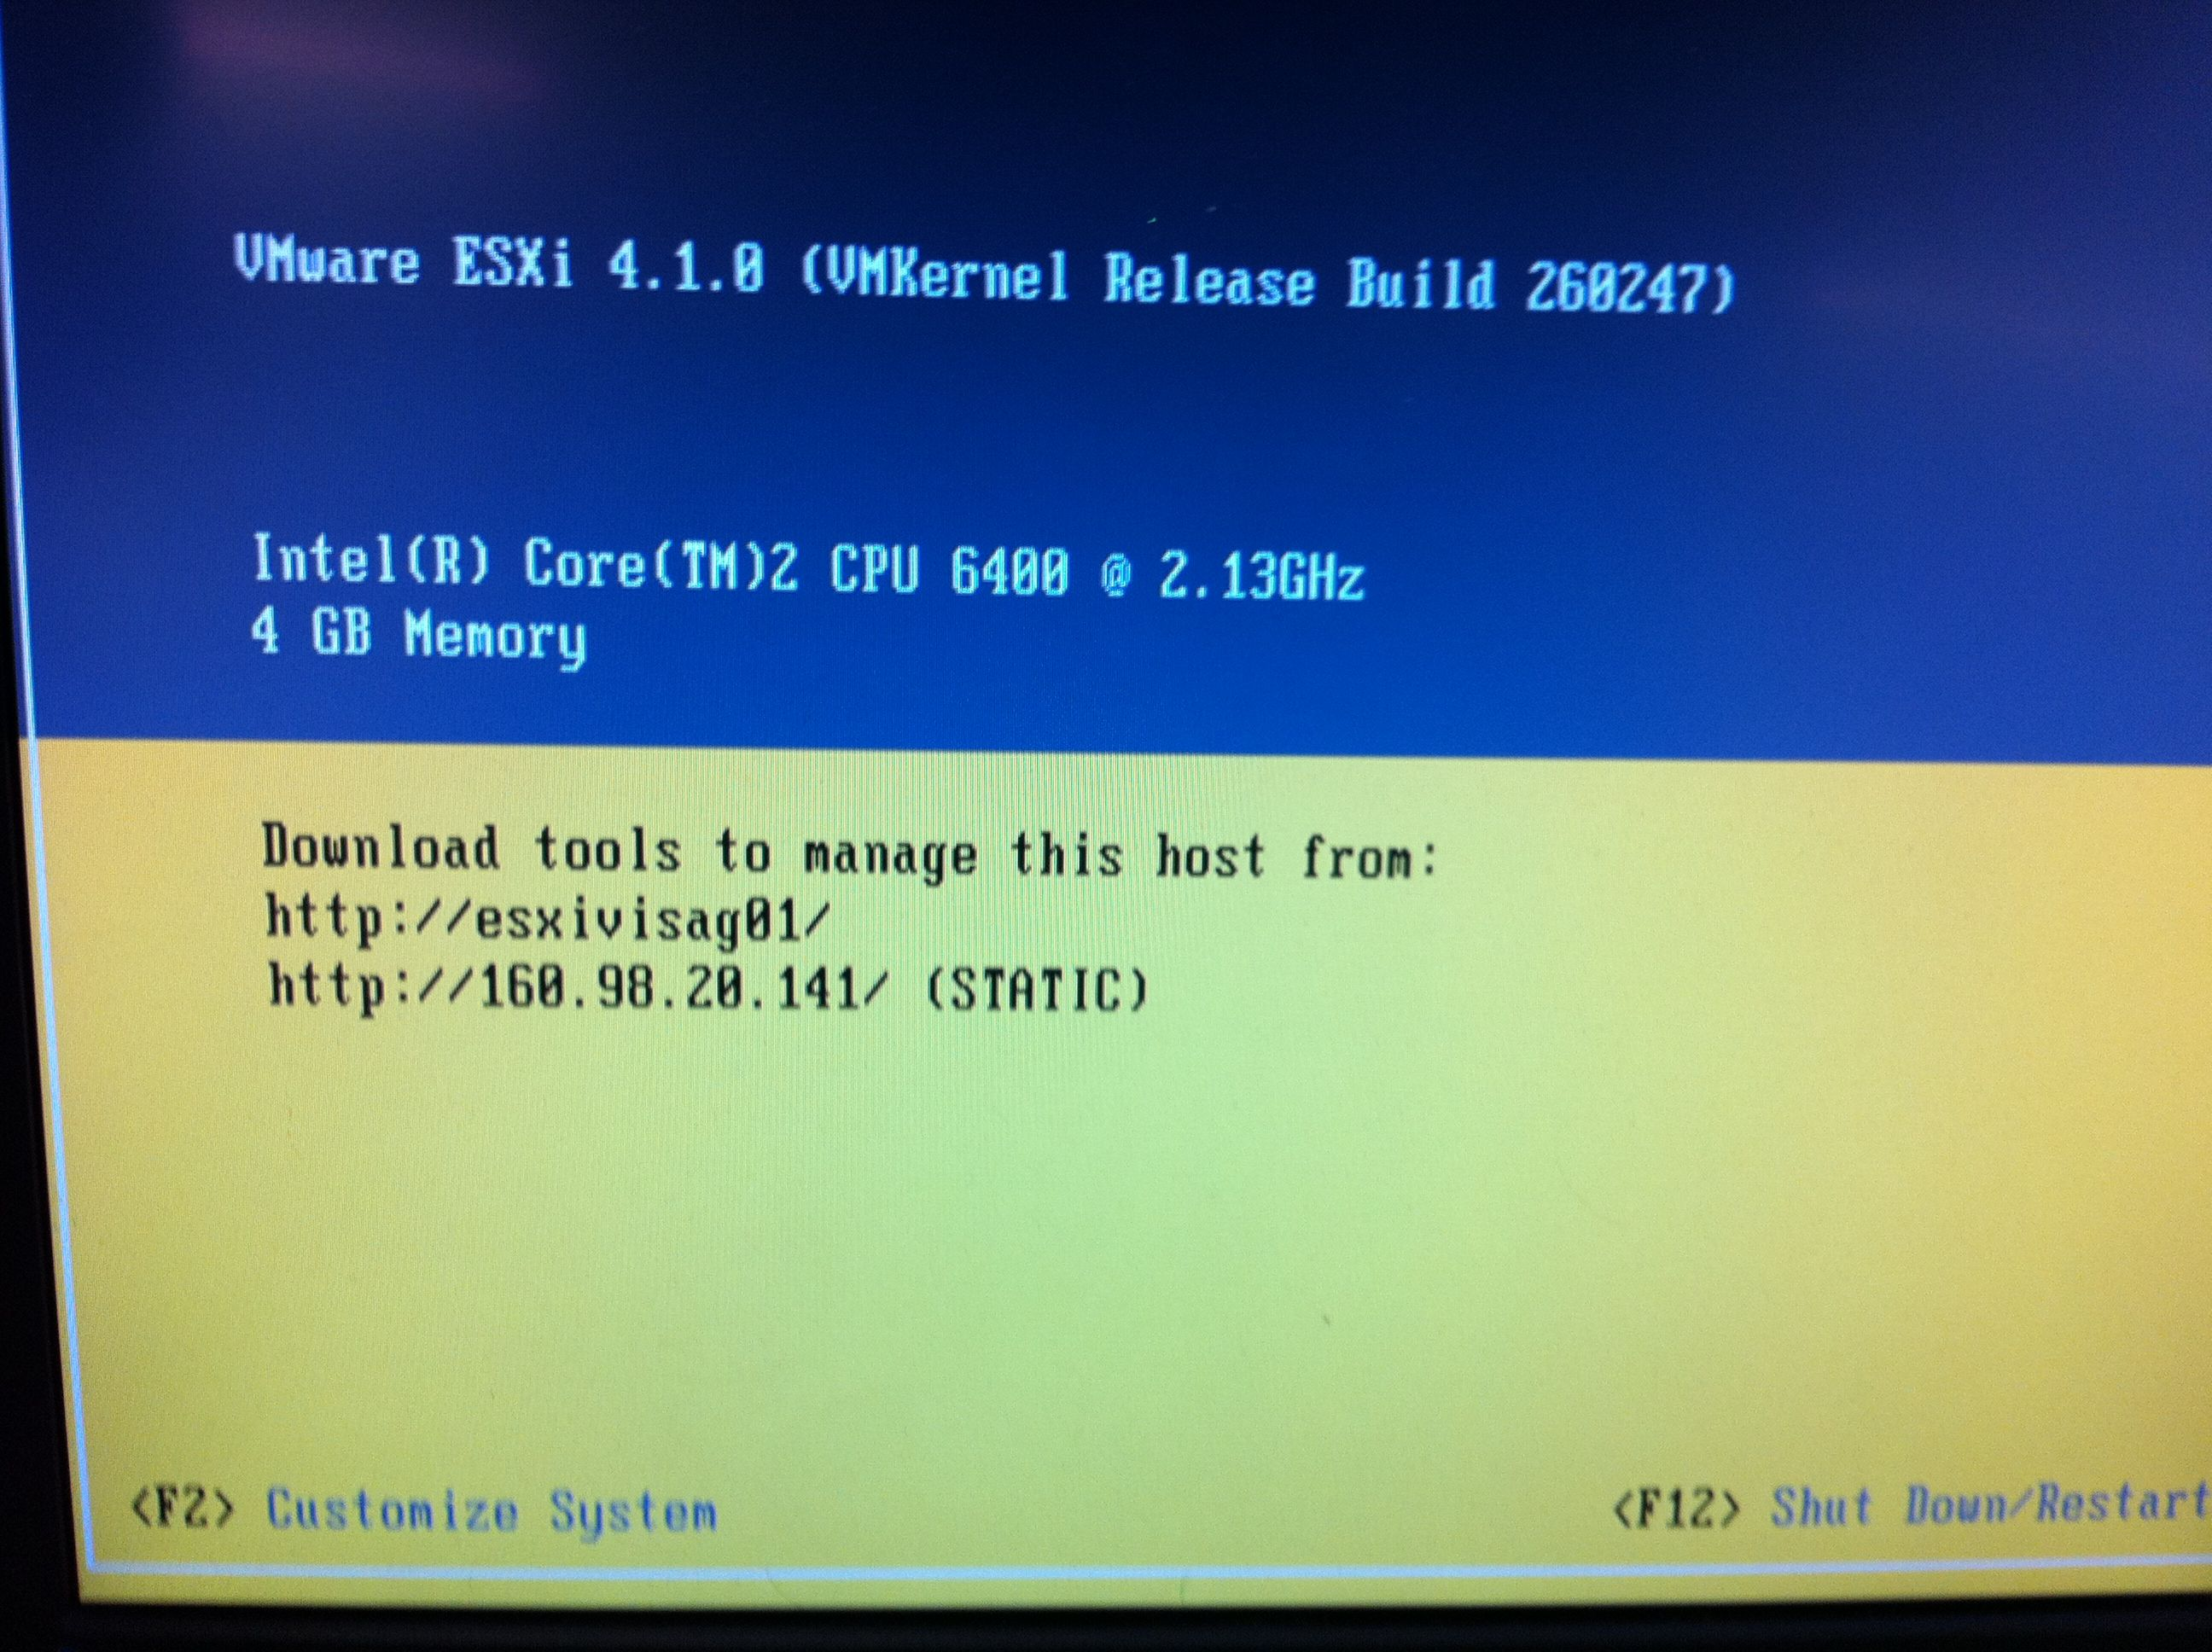
\includegraphics[width=0.5\textwidth]{./pic/esxi_7.jpg}
	\label{fig:esxi_first_screen}
\end{figure}

If a password is already set up, a login screen will appear like in Figure \ref{fig:esxi_login}. Just enter the password and press the "Enter key".
\begin{figure}[ht]
	\caption{VMware ESXi Login screen}
  	\centering
	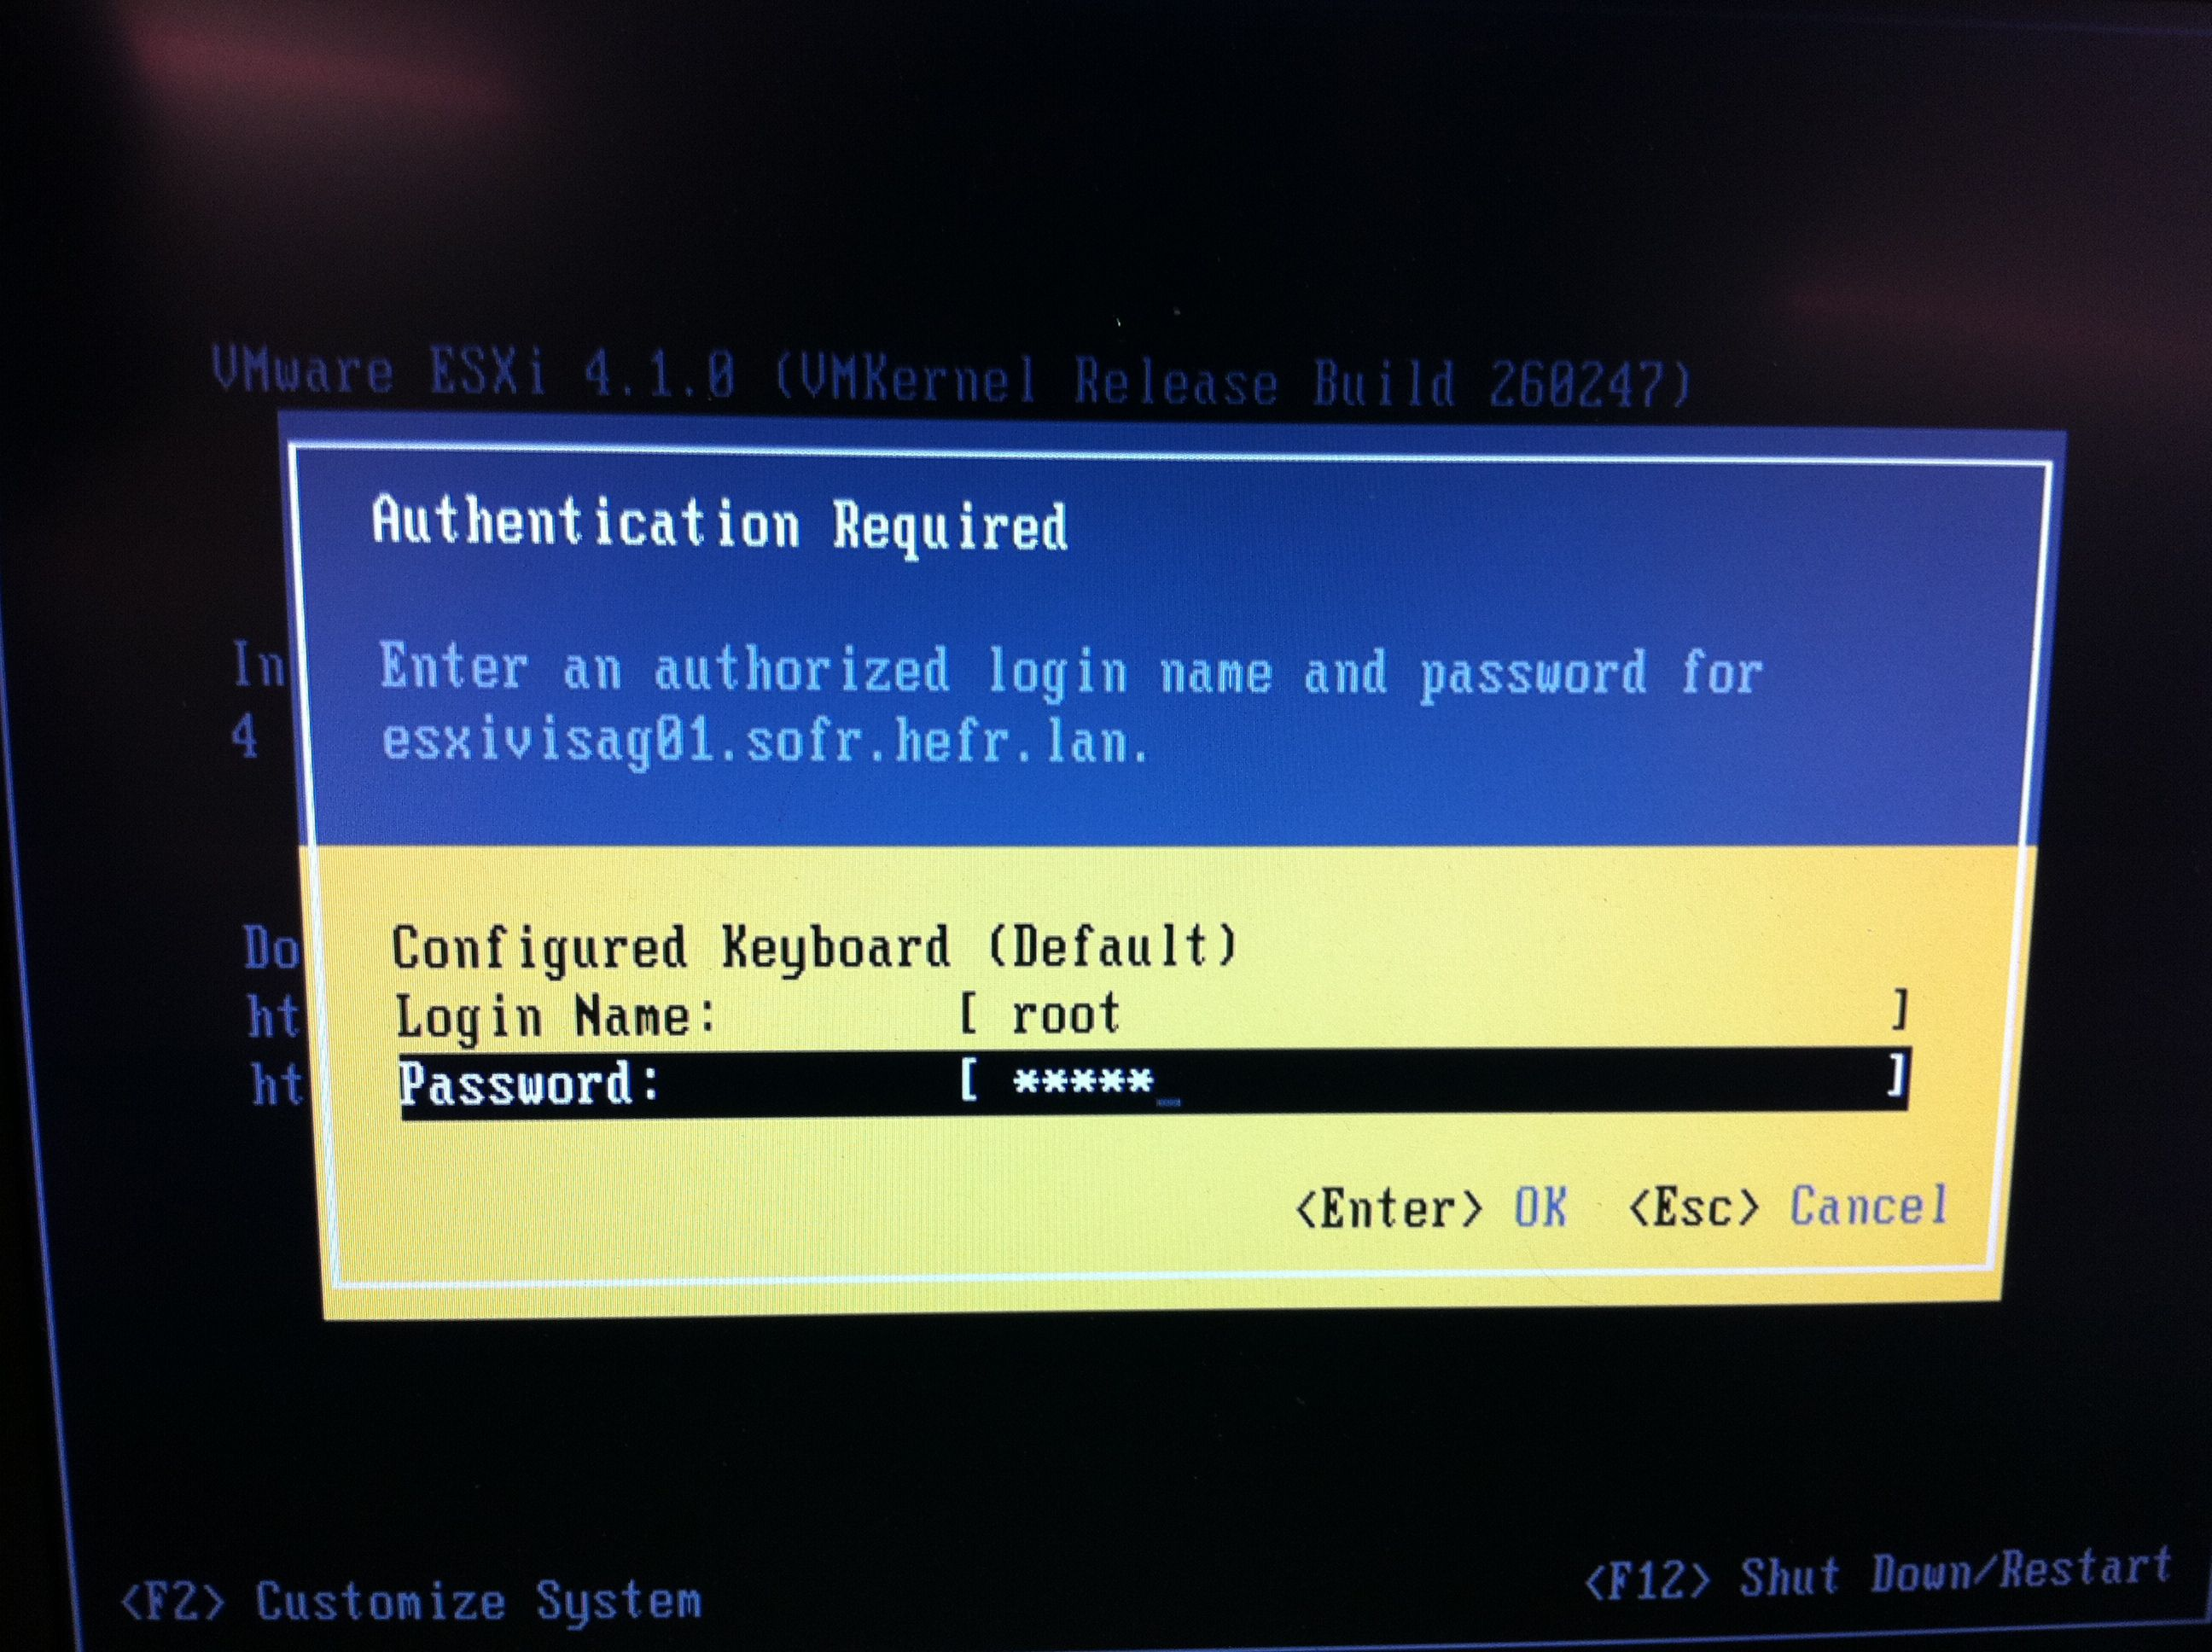
\includegraphics[width=0.5\textwidth]{./pic/esxi_8.jpg}
	\label{fig:esxi_login}
\end{figure}

\pagebreak
\textbf{Network configuration}\\
The ESXi platform needs a static IP address to work well with POP-C++ Virtual. Once logged into the ESXi system, we can modify the IP parameter in the "Configure Management Network" section (see Figure \ref{fig:esxi_sysconf}).

\begin{figure}[ht]
	\caption{VMware ESXi System configuration}
  	\centering
	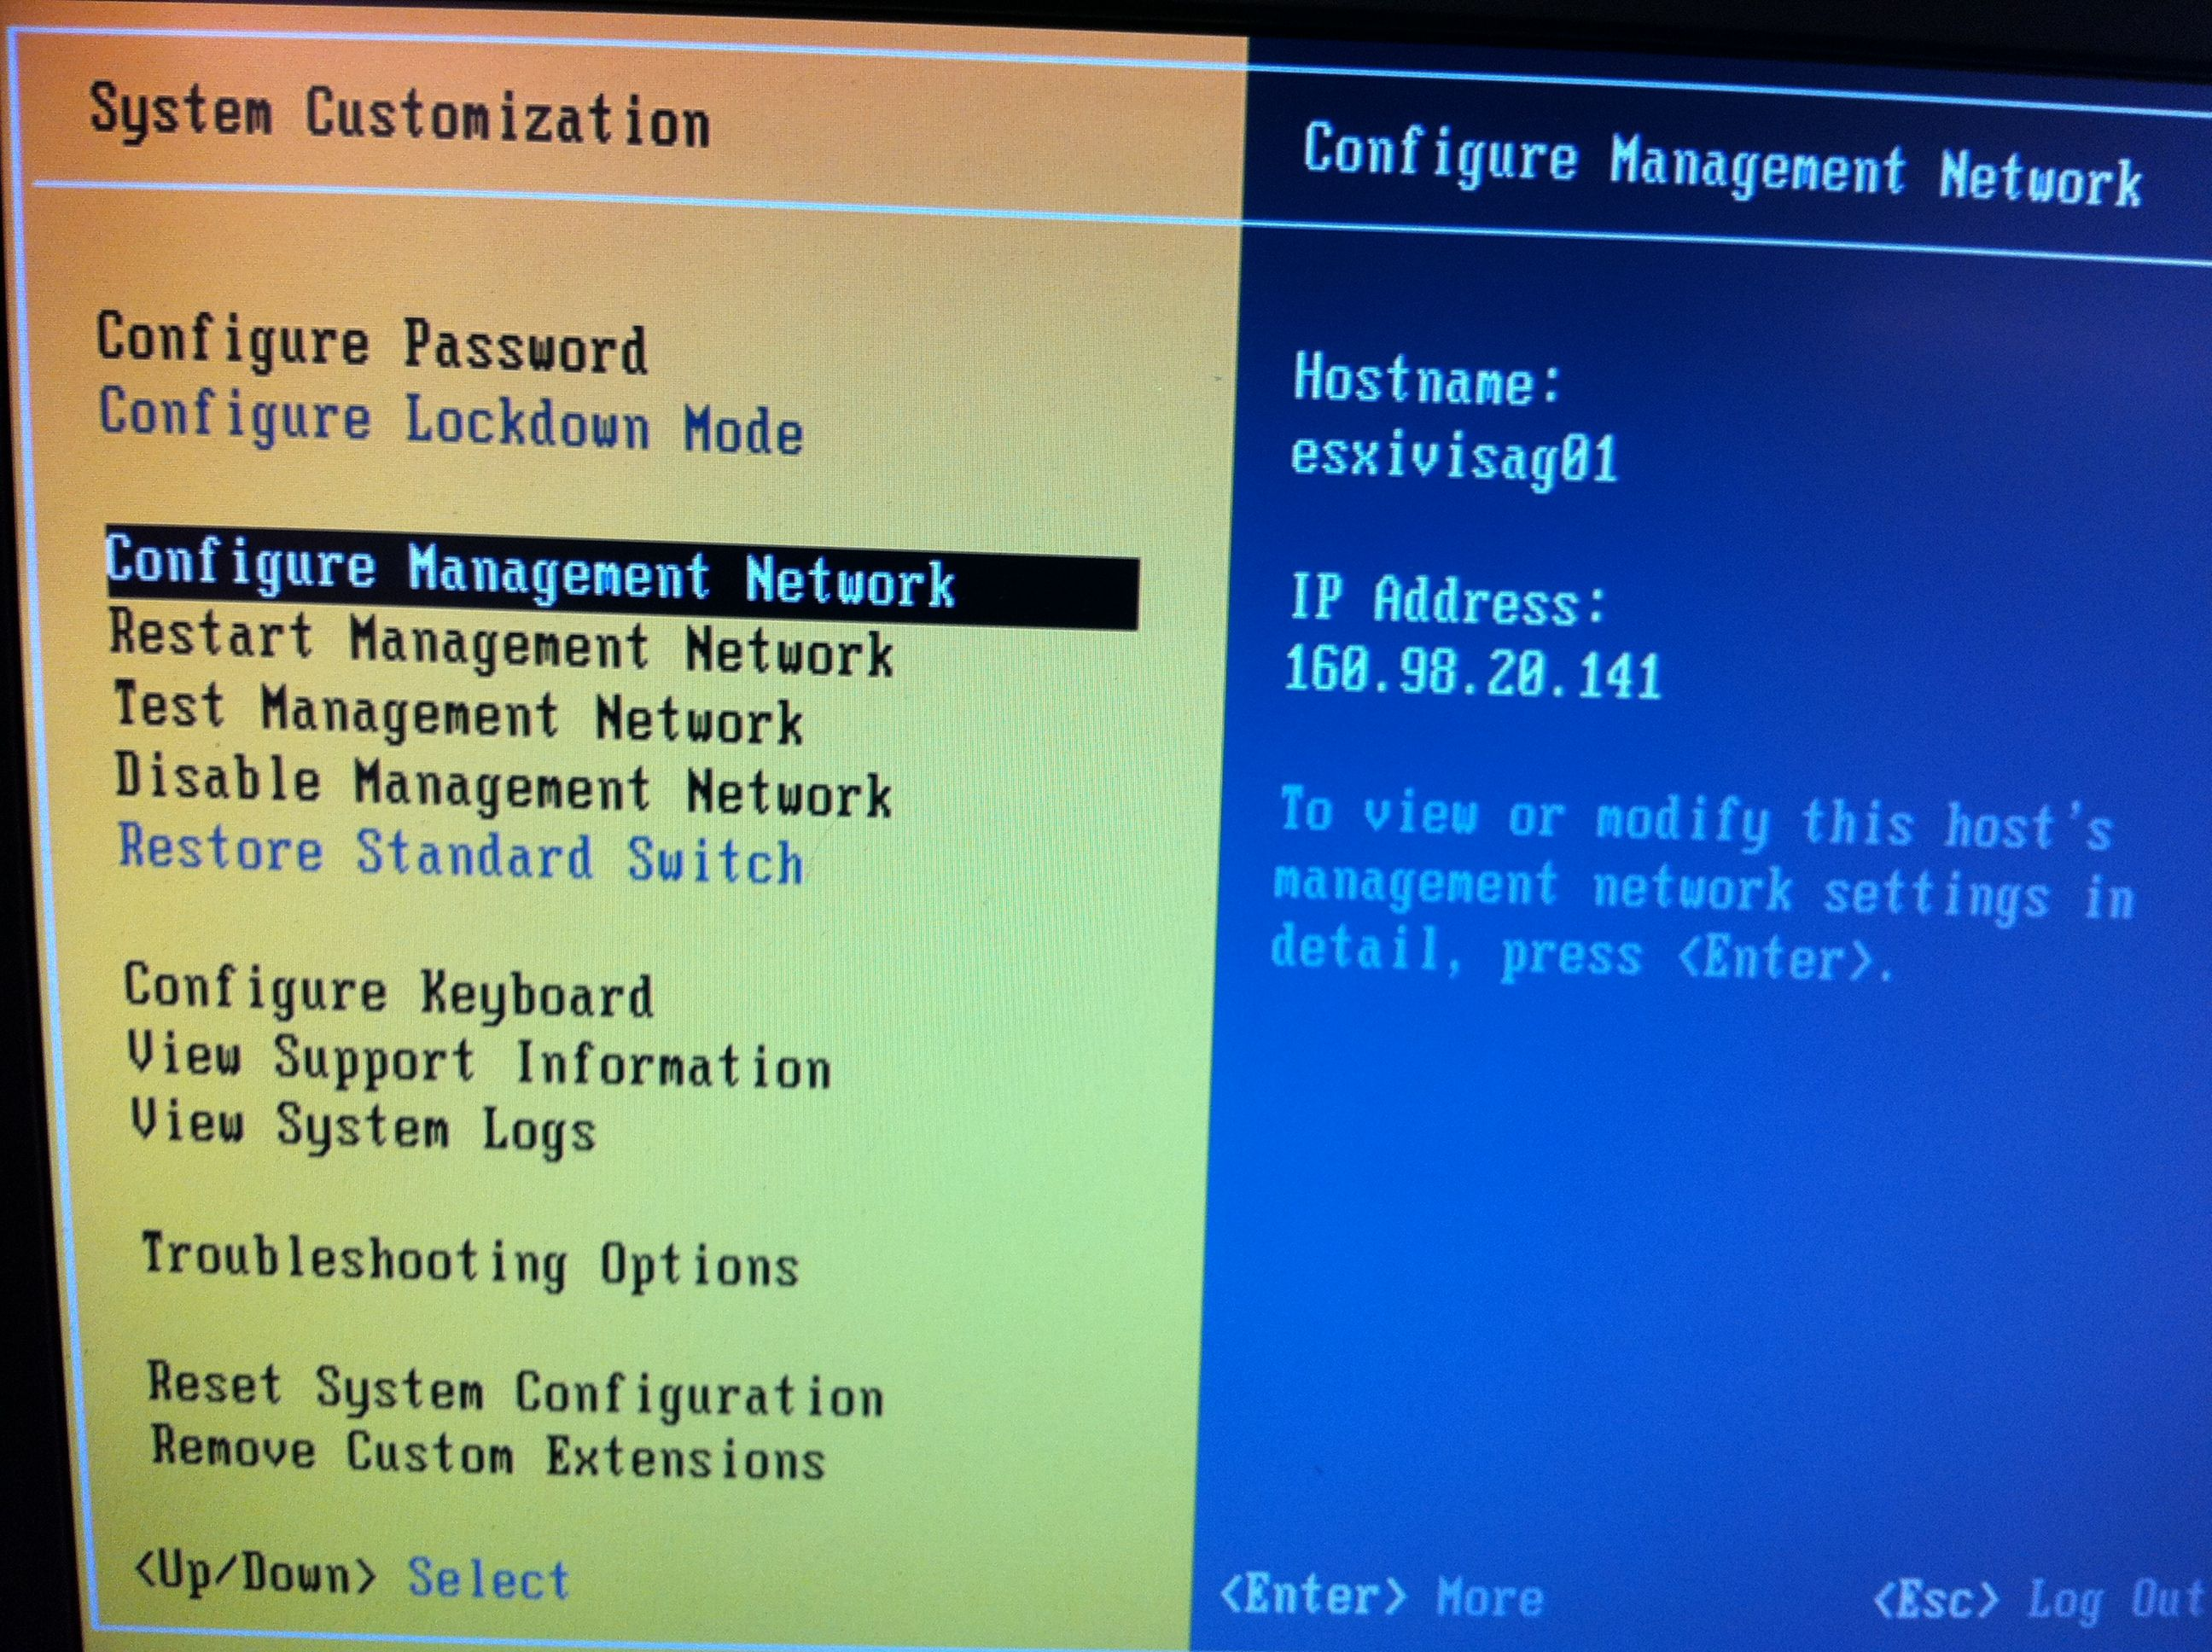
\includegraphics[width=0.5\textwidth]{./pic/esxi_9.jpg}
	\label{fig:esxi_sysconf}
\end{figure}

In the "Configure Management Network" section, we can select the "IP Configuration" subsection to modify the IPv4 parameter (see Figure \ref{fig:esxi_sysconf_ip}).

\begin{figure}[ht]
	\caption{VMware ESXi Network Management Configuration}
  	\centering
	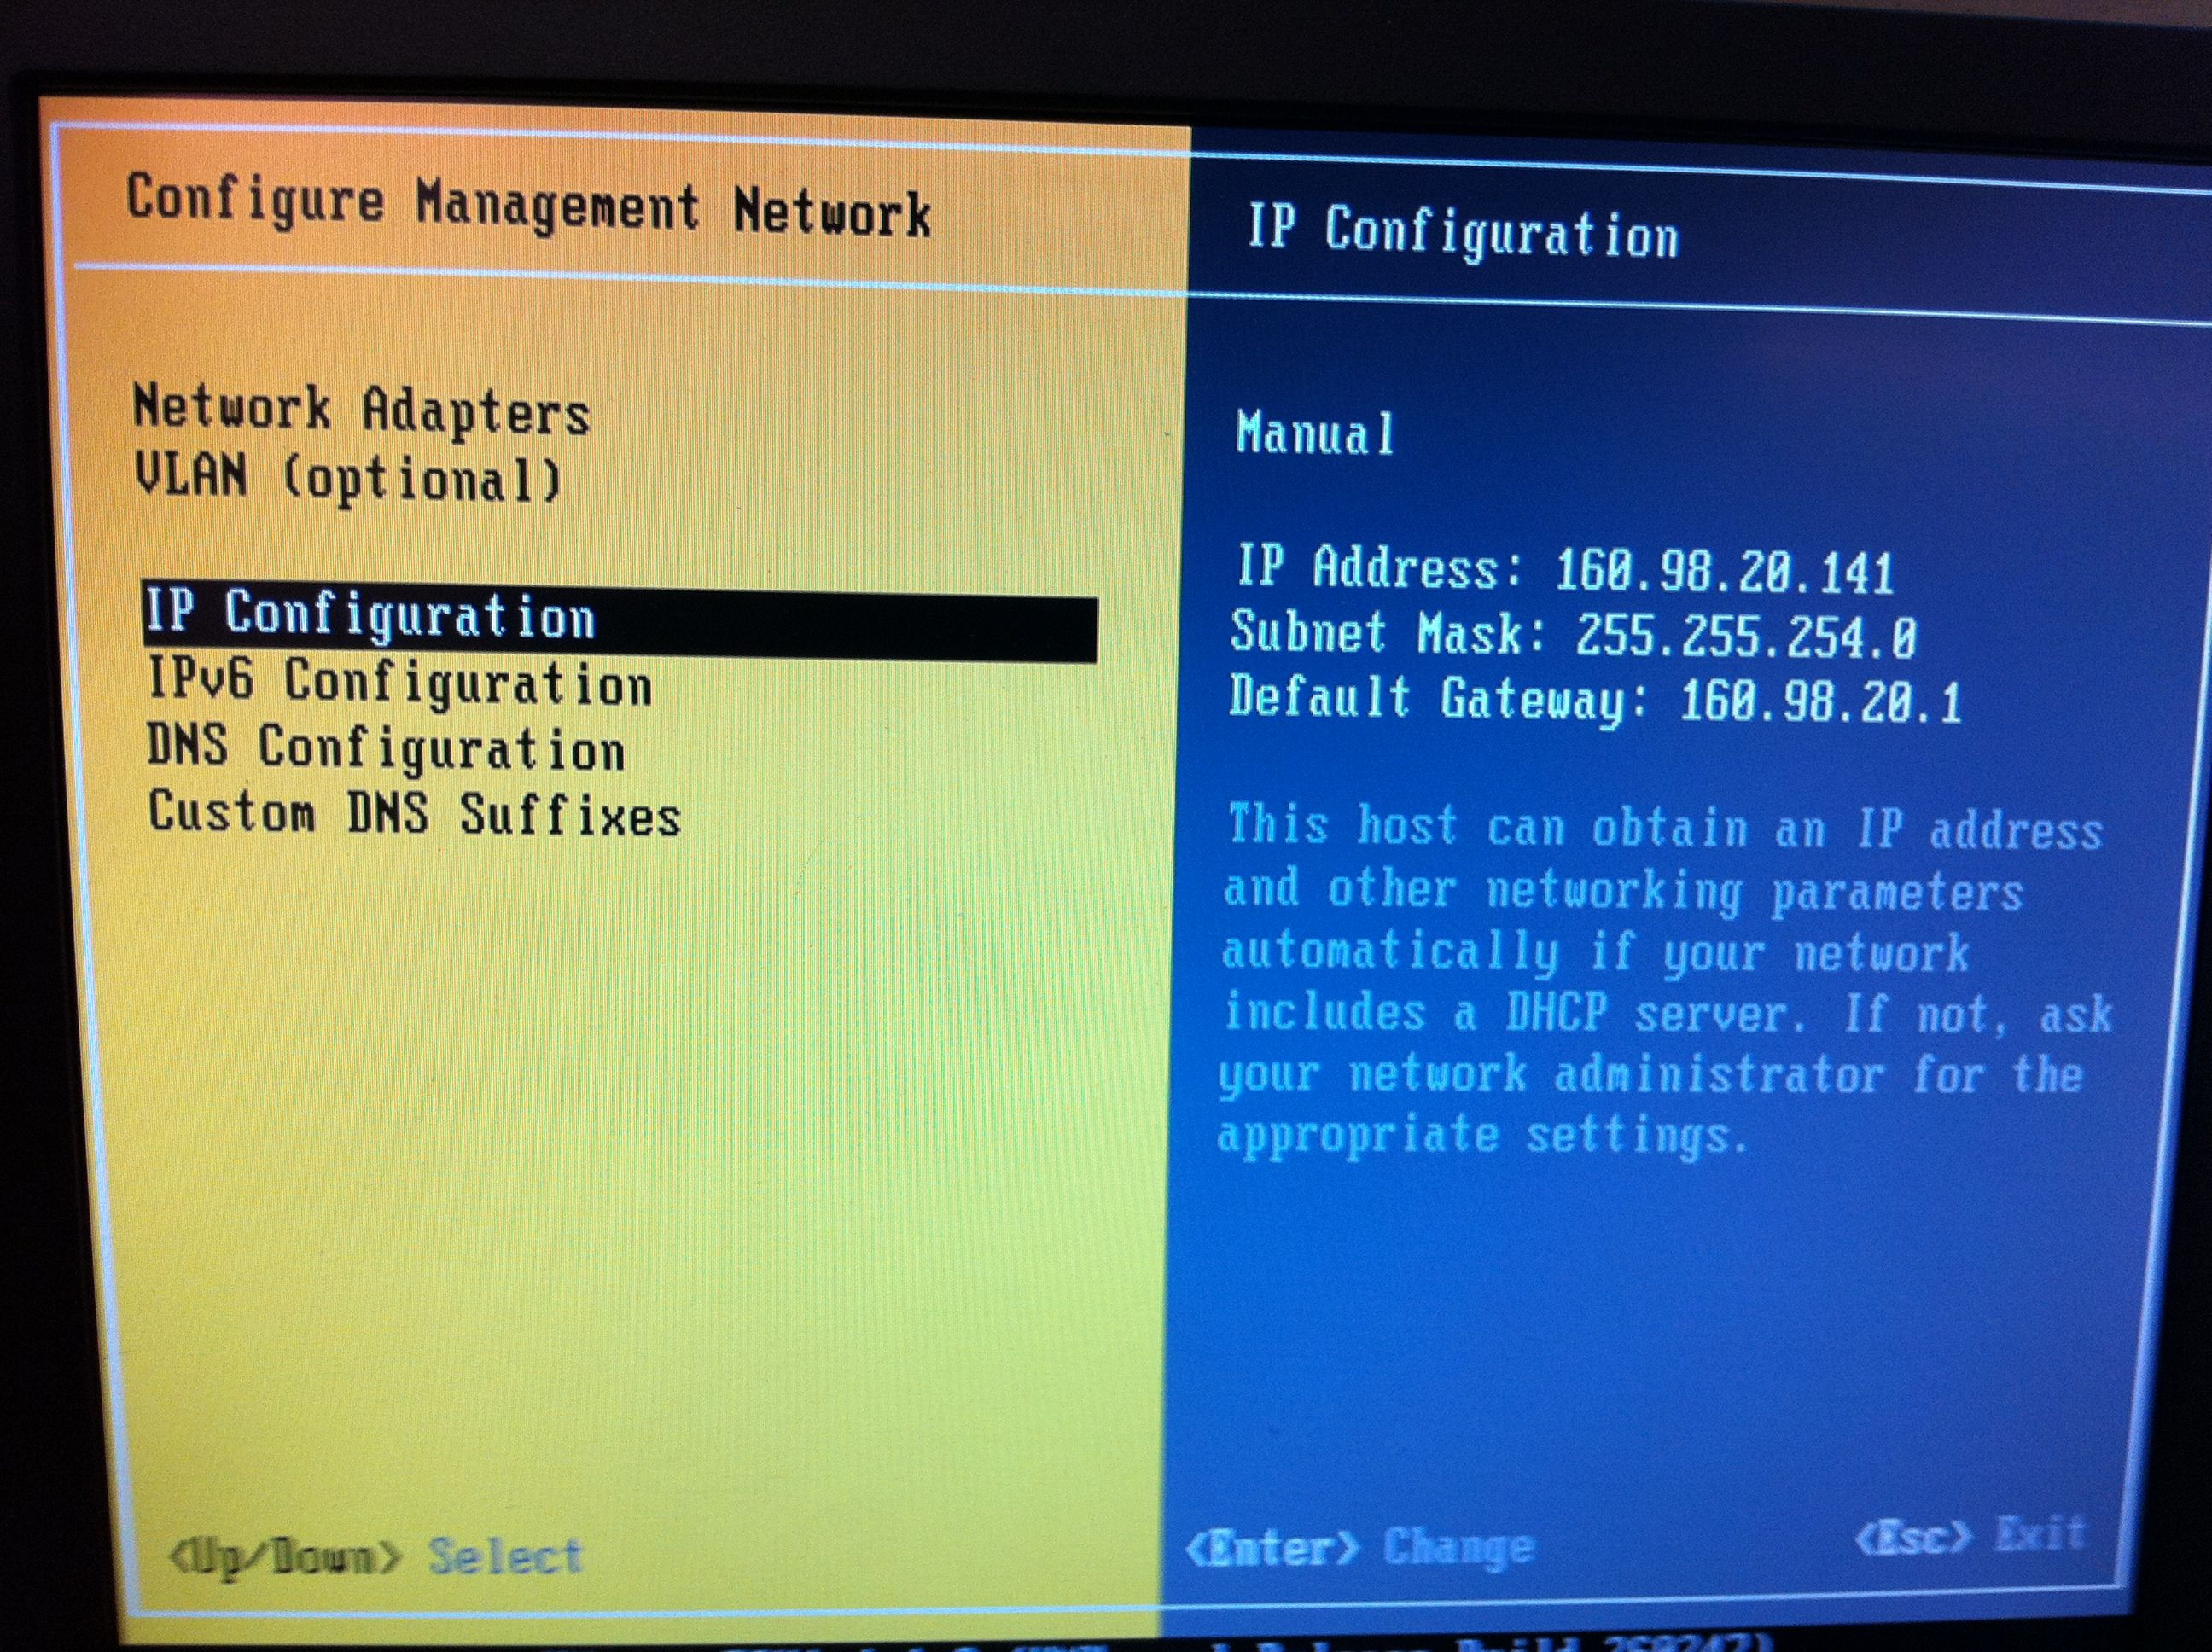
\includegraphics[width=0.5\textwidth]{./pic/esxi_10.jpg}
	\label{fig:esxi_sysconf_ip}
\end{figure}

\pagebreak
Once in the IP Configuration subsection, we can select "Set static IP address and network configuration" and fill the fields below (see Figure \ref{fig:esxi_sysconf_ipv4}). When the information are set, we can save them by pressing the "Enter" key. 

\begin{figure}[ht]
	\caption{VMware ESXi IPv4 Configuration}
  	\centering
	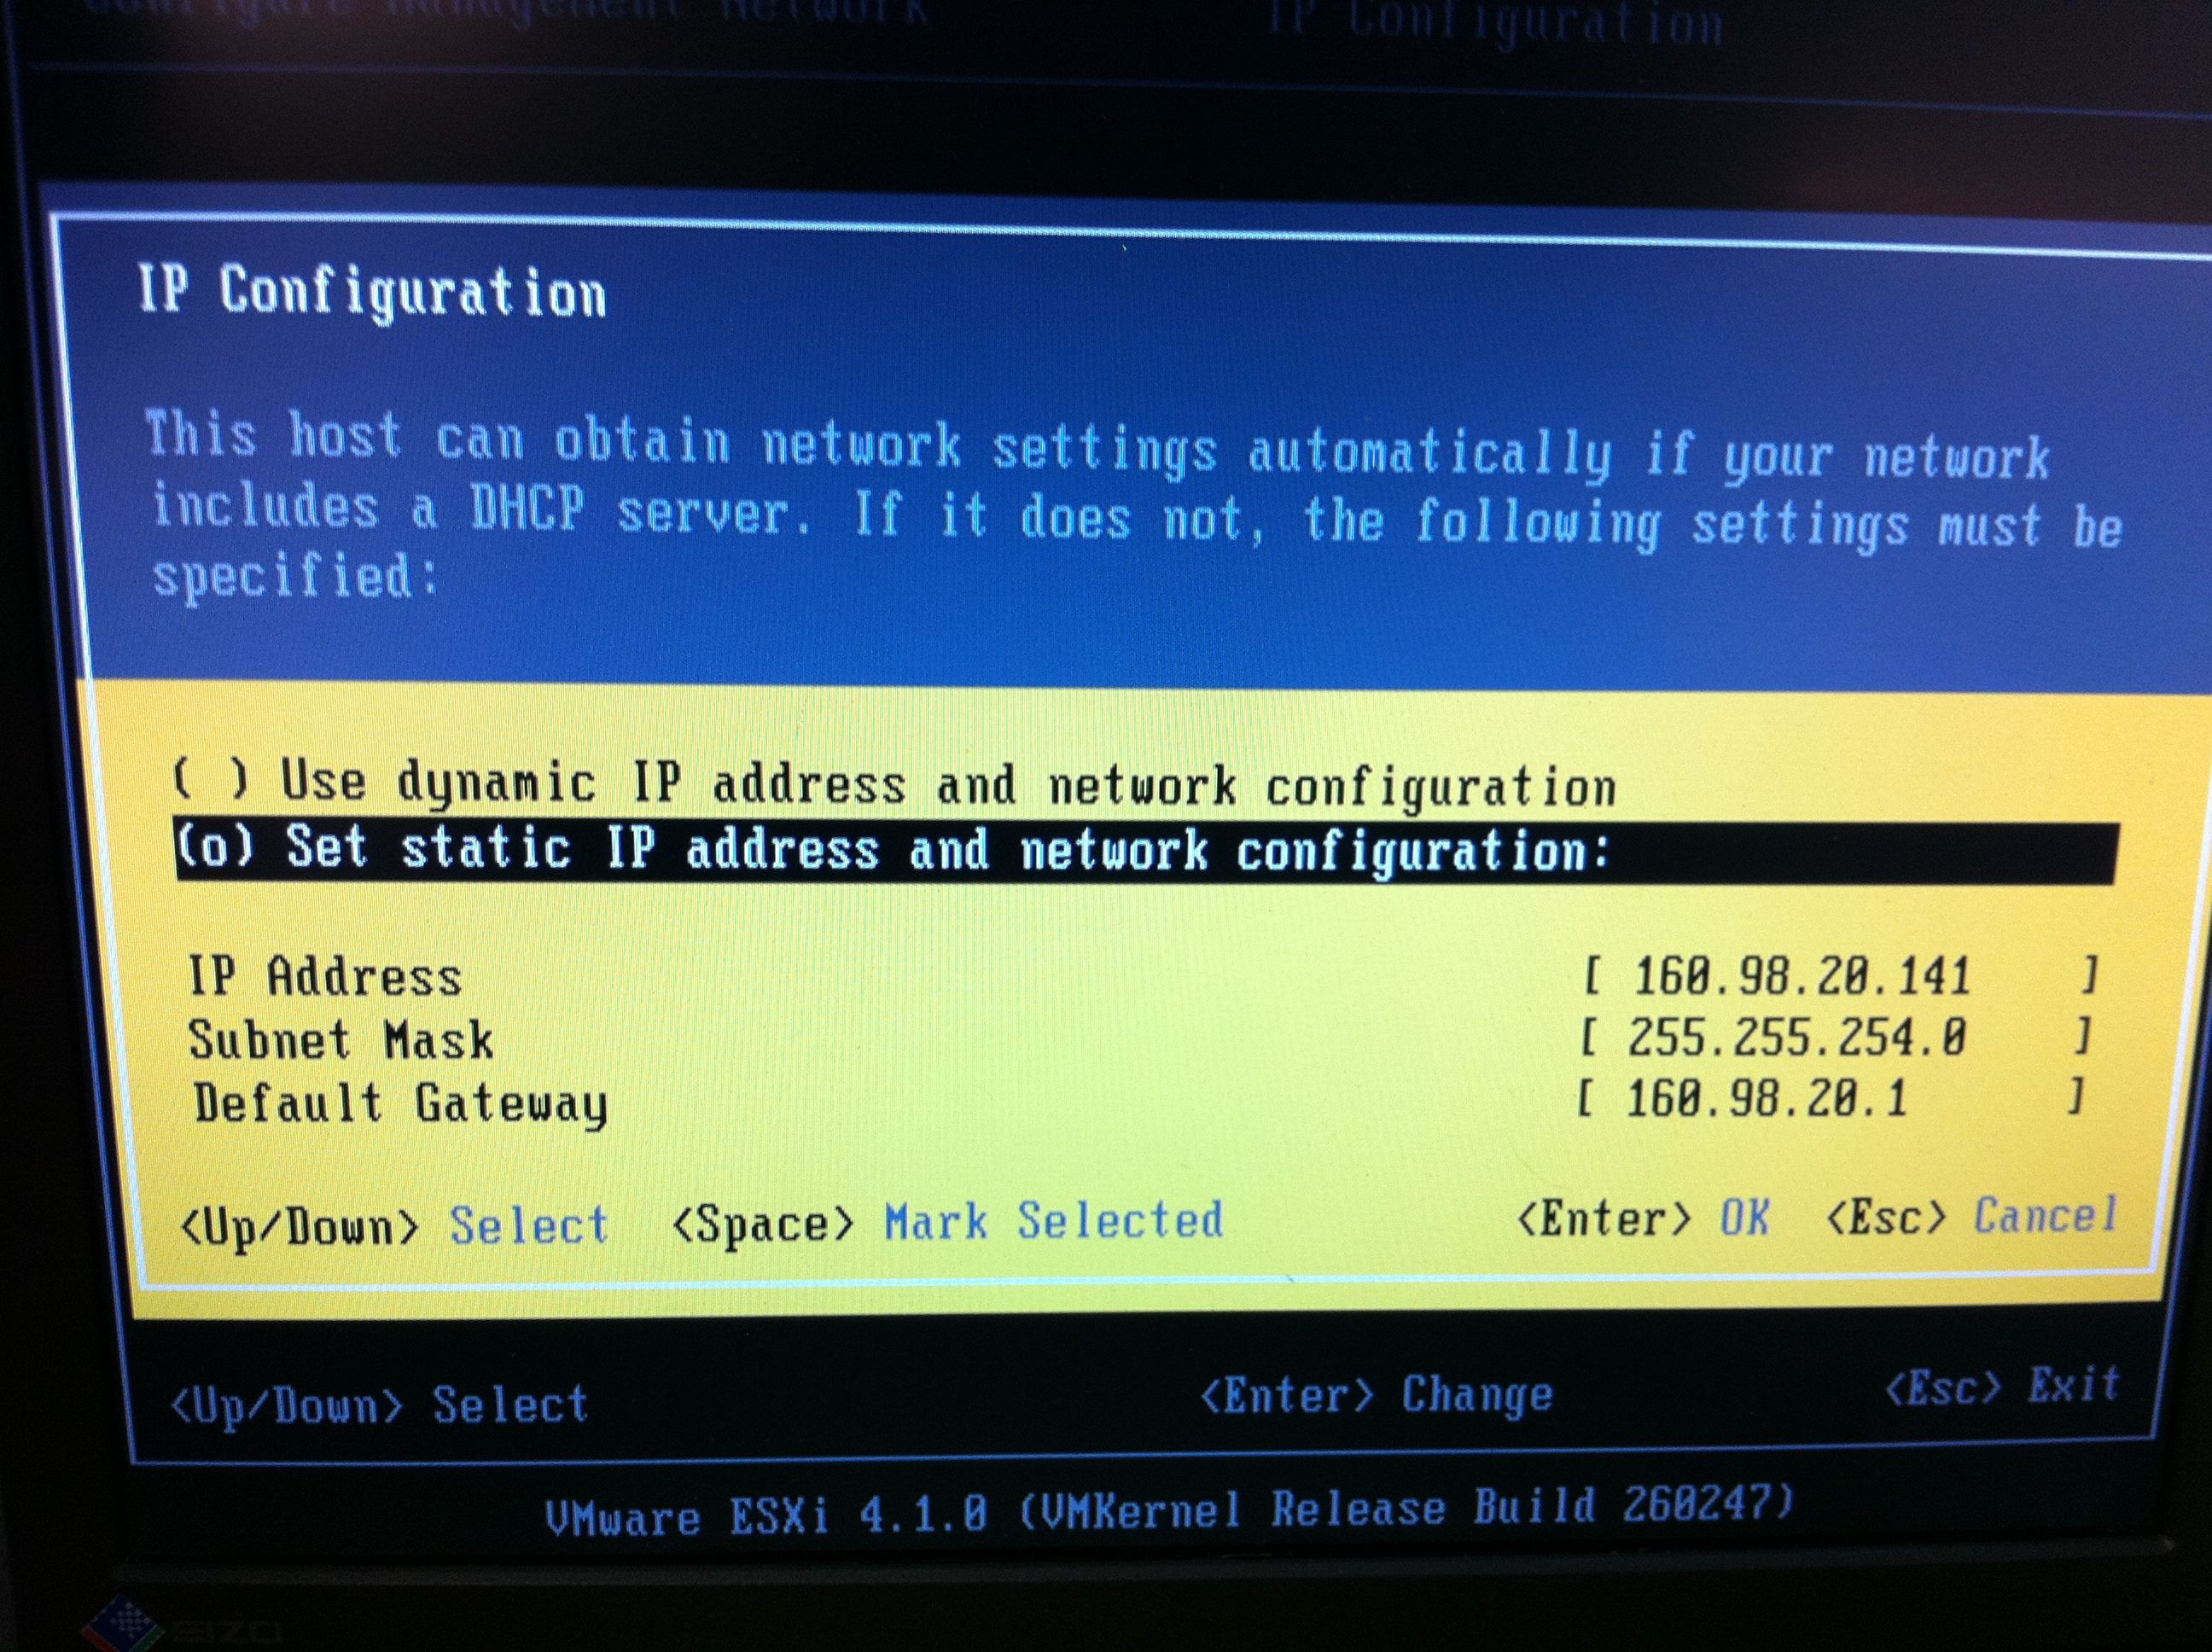
\includegraphics[width=0.5\textwidth]{./pic/esxi_11.jpg}
	\label{fig:esxi_sysconf_ipv4}
\end{figure}


After setting the IPv4 parameters, we need to set up the DNS parameter. In the "Configure Management Network", we will choose "DNS configuration" instead of "IP configuration" (see Figure \ref{fig:esxi_sysconf_ip}). Like in Figure \ref{fig:esxi_sysconf_dns}, we select "Use the following DNS server addresses and hostname" and fill the fields. \s

\textit{NOTE:} This step is not mandatory if you have a unique DNS name attributed by IP address. But your ESXi host must be reachable by its DNS hostname. 
\begin{figure}[ht]
	\caption{VMware ESXi System configuration}
  	\centering
	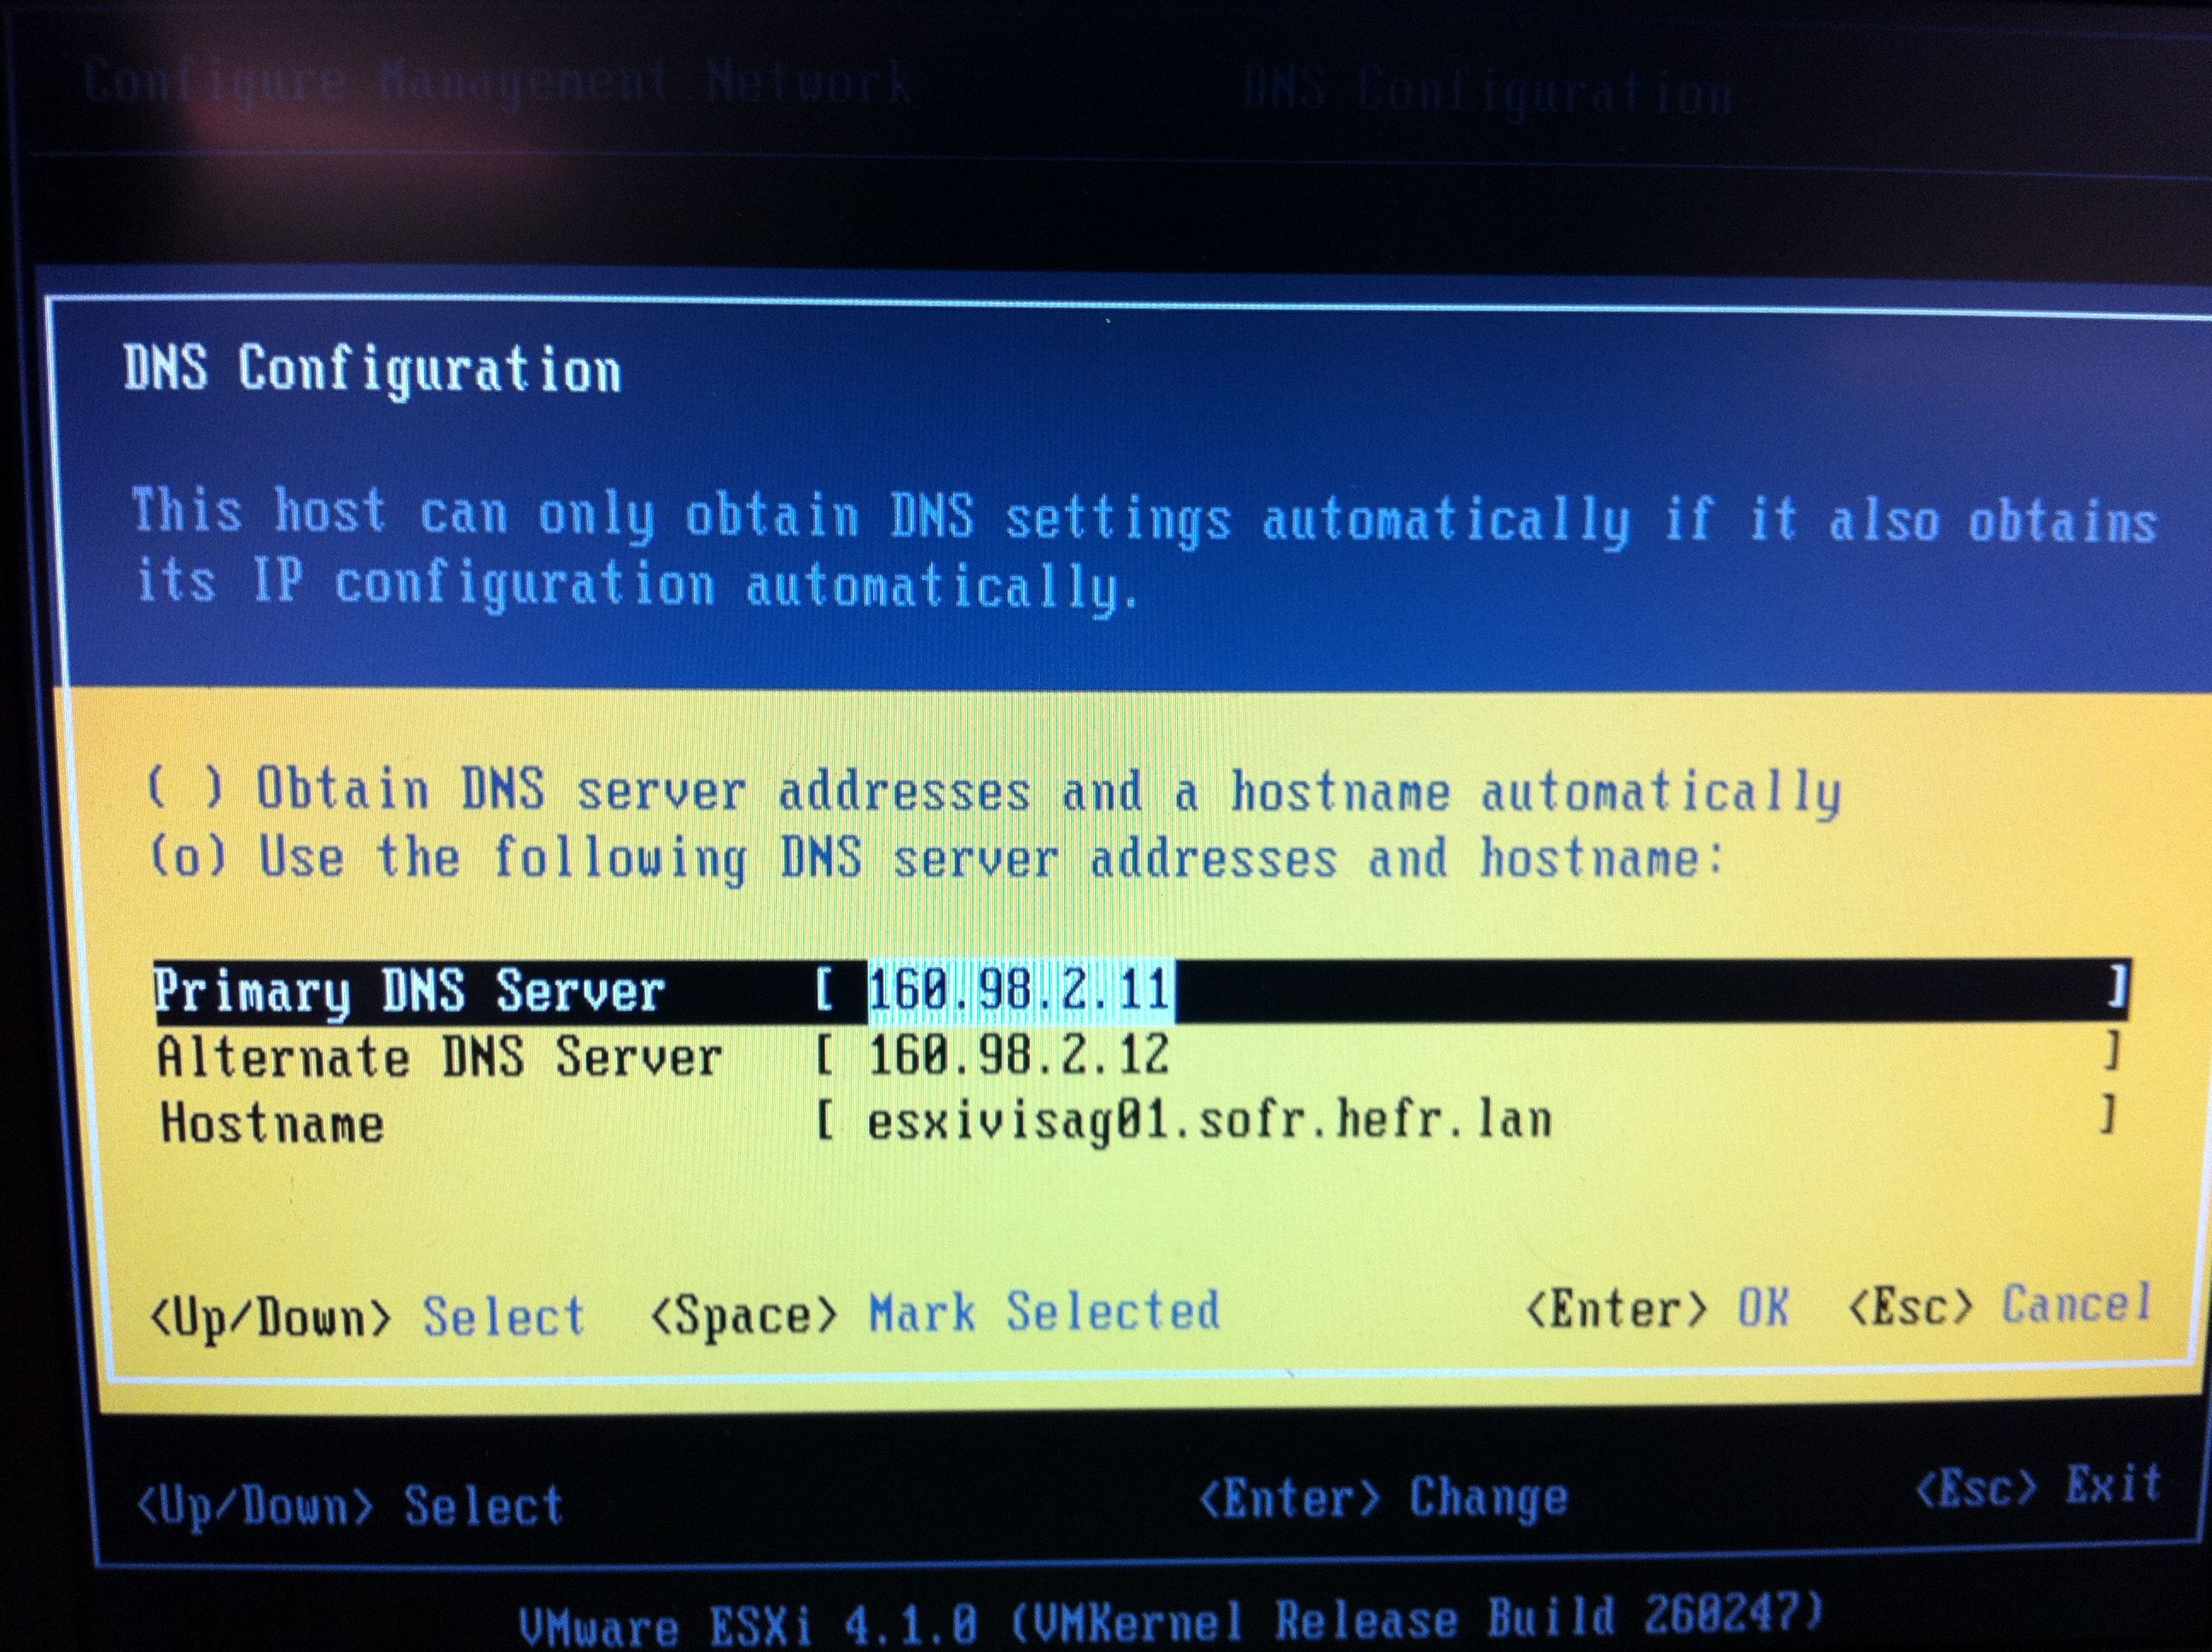
\includegraphics[width=0.5\textwidth]{./pic/esxi_12.jpg}
	\label{fig:esxi_sysconf_dns}
\end{figure}

\pagebreak

\textbf{Password configuration}\\
To set or change the administrator password, we will choose "Configure Password" in the ESXi System Configuration (see Figure \ref{fig:esxi_sysconf}). A screen will be prompted (Figure \ref{fig:esxi_sysconf_pass}) and we just need to fill it. 
\begin{figure}[ht]
	\caption{VMware ESXi System configuration}
  	\centering
	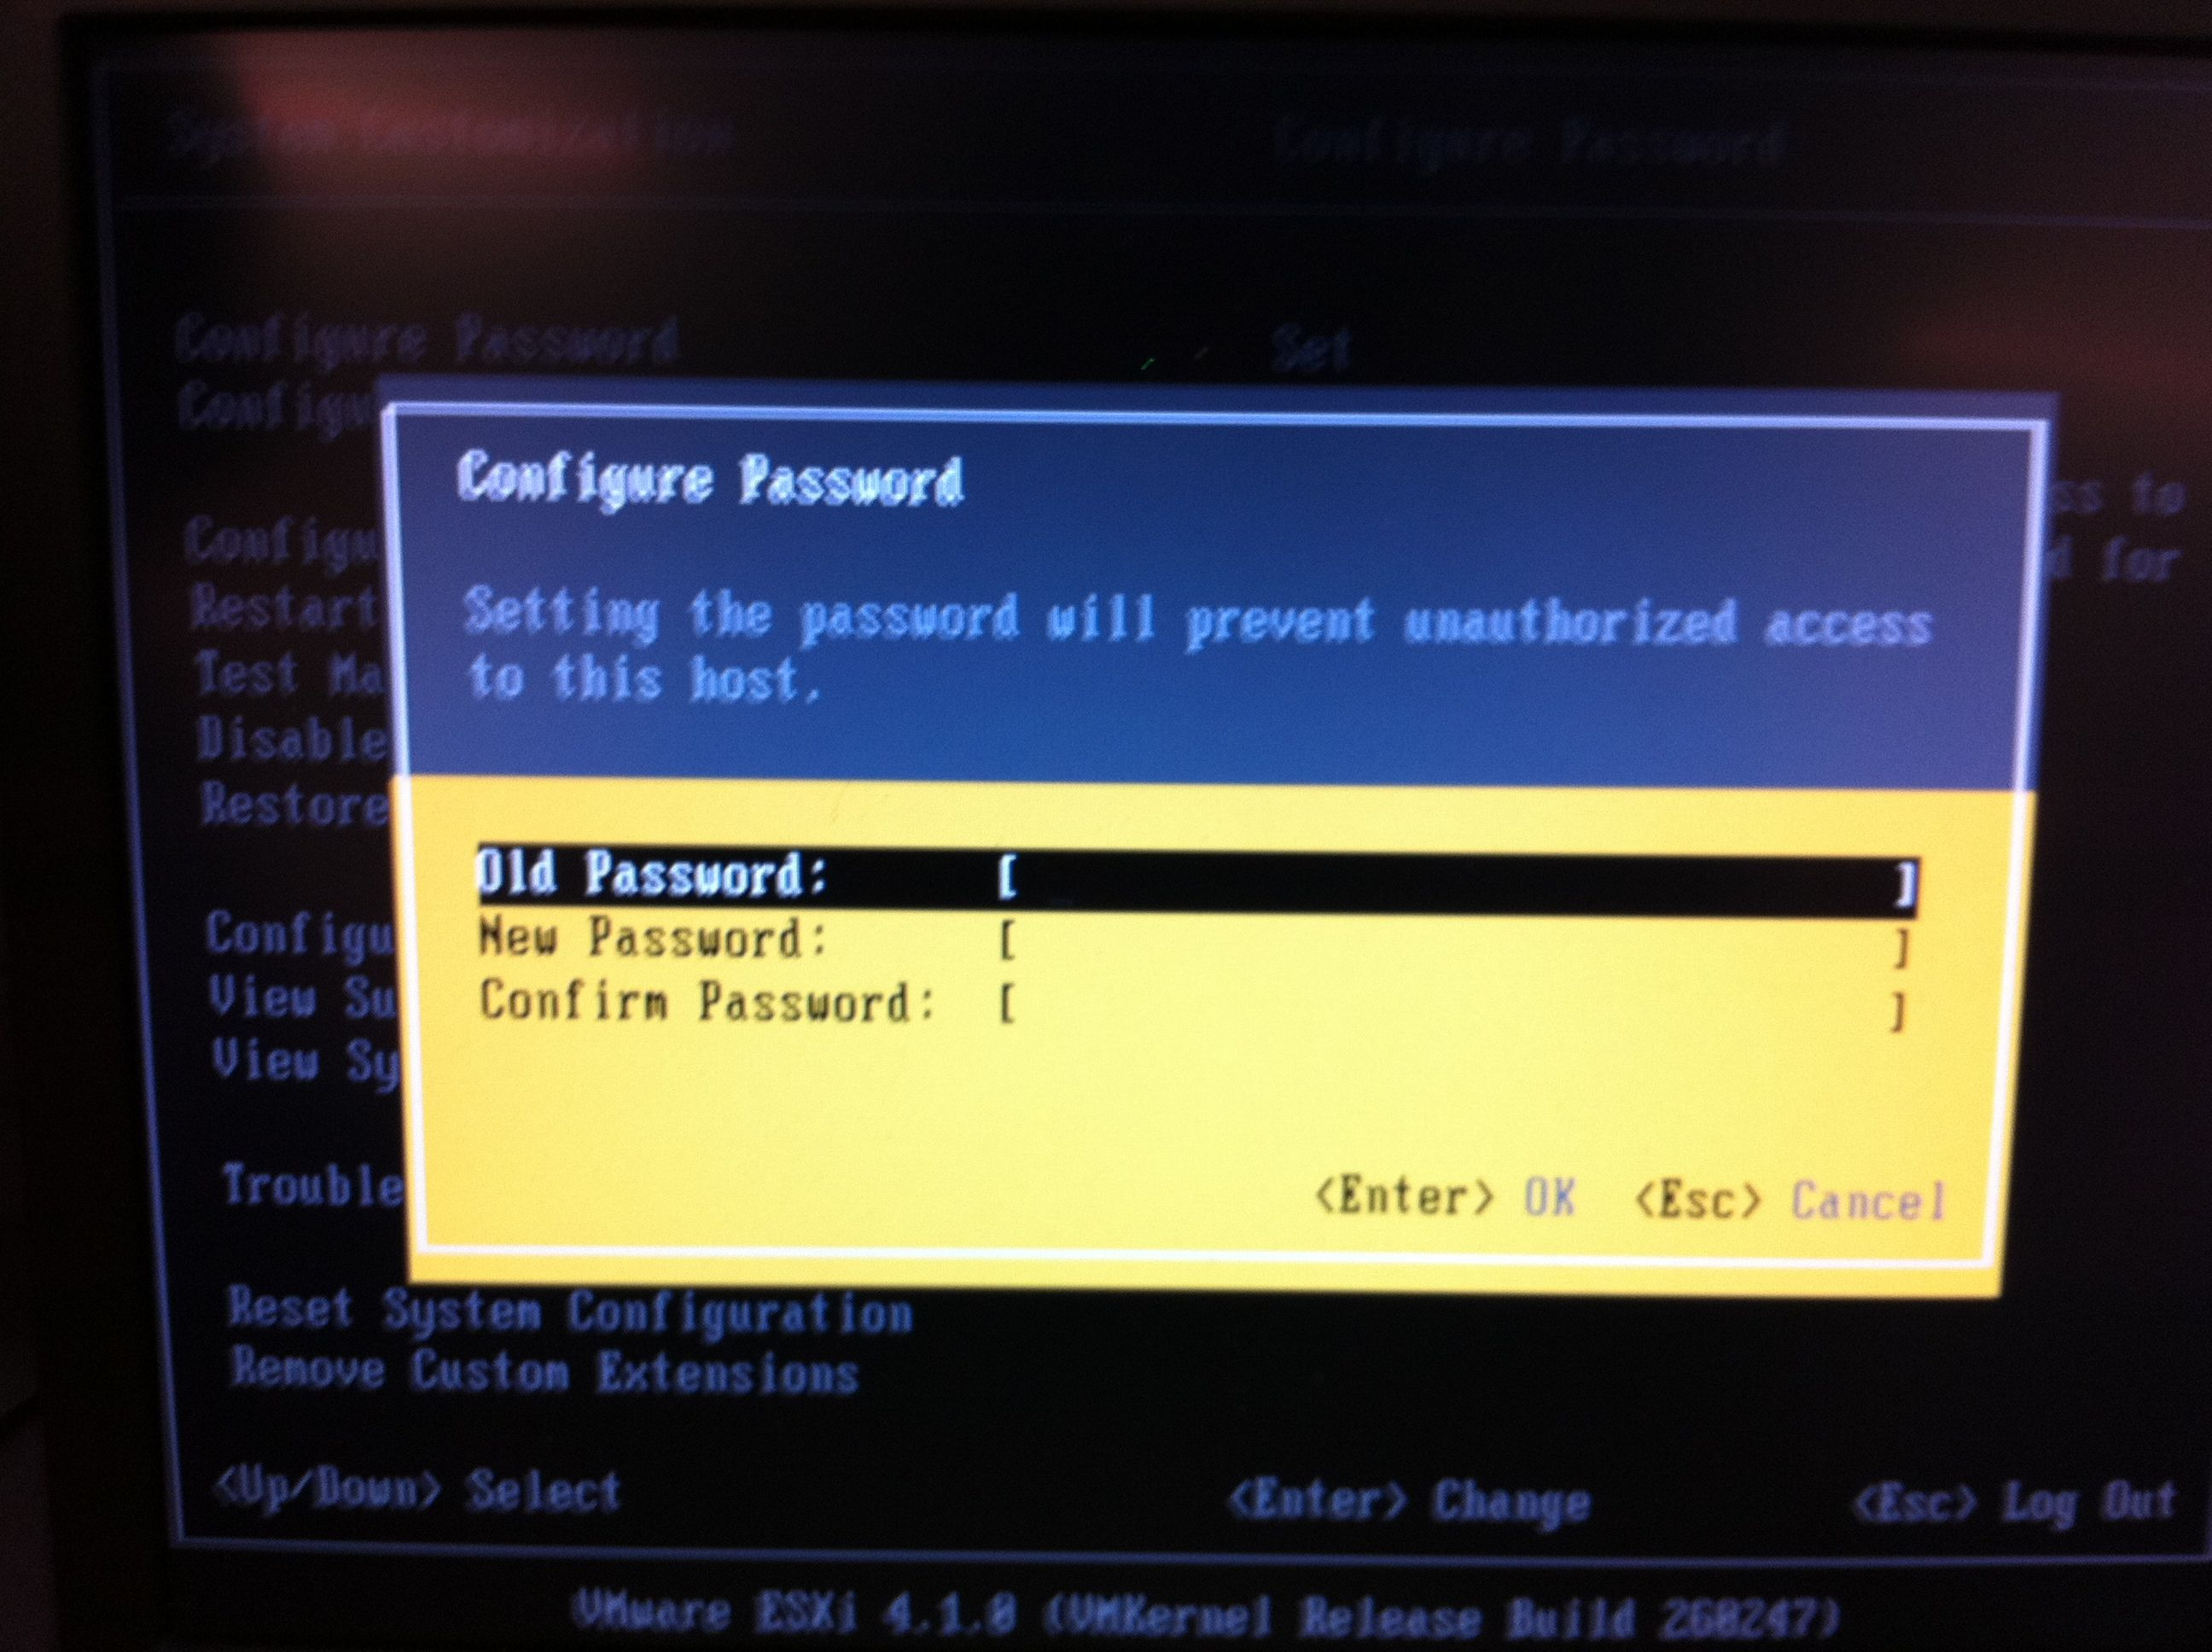
\includegraphics[width=0.5\textwidth]{./pic/esxi_13.jpg}
	\label{fig:esxi_sysconf_pass}
\end{figure}


%---------------
% CREATE VM ON VSPHERE
%---------------
\section{Create a VM with vSphere 4.1}
\label{app:createvm}

Before installing a VM, we need to create it with the vSphere Client. On the item symbolising the ESXi node just right-click and choose "New Virtual Machine...". 

\begin{figure}[ht]
	\caption{vSphere Client - Create VM (Step 1)}
  	\centering
	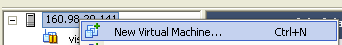
\includegraphics[width=0.5\textwidth]{./pic/createvm_1.png}
	\label{fig:createvm_1}
\end{figure}
\pagebreak


Choose "Typical" configuration and click "Next".
\begin{figure}[ht]
	\caption{vSphere Client - Create VM (Step 2)}
  	\centering
	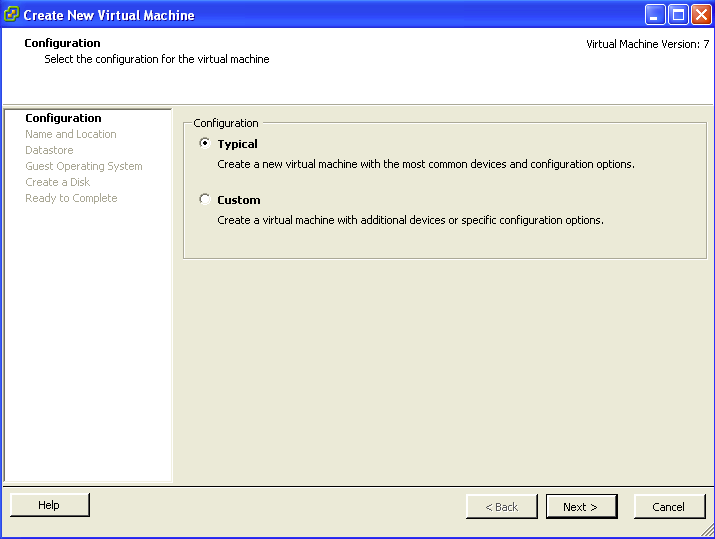
\includegraphics[width=0.5\textwidth]{./pic/createvm_2.png}
	\label{fig:createvm_2}
\end{figure}

Give a name to the VM and click "Next".
\begin{figure}[ht]
	\caption{vSphere Client - Create VM (Step 3)}
  	\centering
	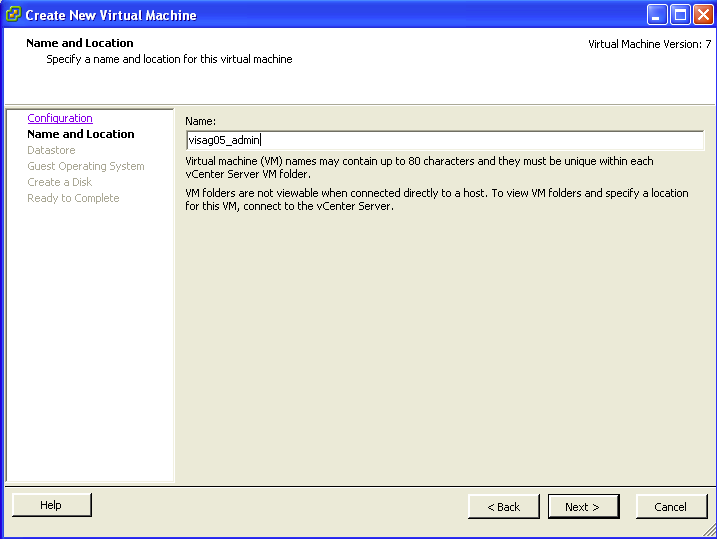
\includegraphics[width=0.5\textwidth]{./pic/createvm_3.png}
	\label{fig:createvm_3}
\end{figure}

\pagebreak
Choose the datastore of destination and click "Next".
\begin{figure}[ht]
	\caption{vSphere Client - Create VM (Step 4)}
  	\centering
	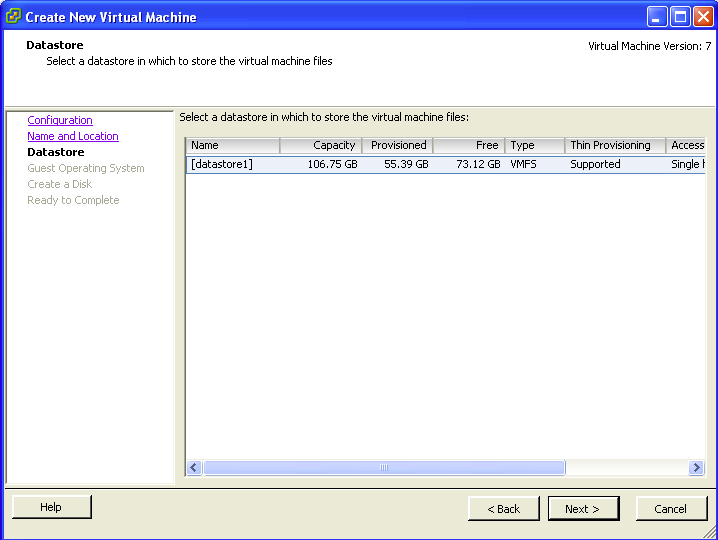
\includegraphics[width=0.5\textwidth]{./pic/createvm_4.png}
	\label{fig:createvm_4}
\end{figure}

Choose the "Operating System" and click "Next".
\begin{figure}[ht]
	\caption{vSphere Client - Create VM (Step 5)}
  	\centering
	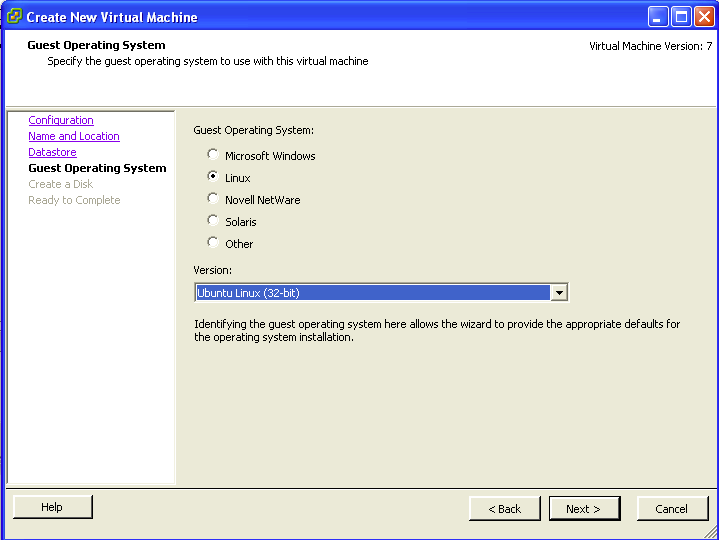
\includegraphics[width=0.5\textwidth]{./pic/createvm_5.png}
	\label{fig:createvm_5}
\end{figure}

\pagebreak
Choose the size of the disk and select "Allocate and commit ..." and click "Next".
\begin{figure}[ht]
	\caption{vSphere Client - Create VM (Step 6)}
  	\centering
	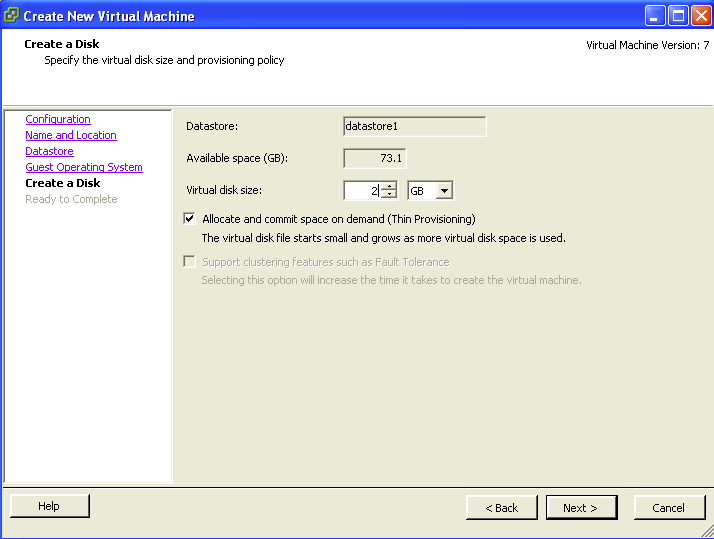
\includegraphics[width=0.5\textwidth]{./pic/createvm_6.png}
	\label{fig:createvm_6}
\end{figure}

Click "Finish", the VM is created and appears in the left-side of the vSphere client. 
\begin{figure}[ht]
	\caption{vSphere Client - Create VM (Step 7)}
  	\centering
	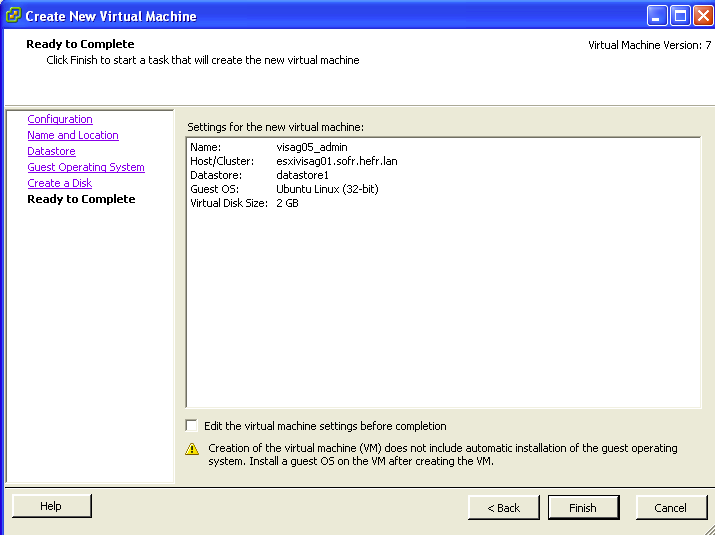
\includegraphics[width=0.5\textwidth]{./pic/createvm_7.png}
	\label{fig:createvm_7}
\end{figure}


\pagebreak
%---------------
% CREATE A SNAPSHOT
%---------------
\section{Create a snapshot of a VM}
\label{app:snap}
The worker VM will be reverted to a snapshot before executing a job. To be able to do this action, we need to create the snapshot of our worker VM in the good state. After installing all the needed elements, you should release the dhcp lease and shutdown the VM. On a Ubuntu OS, use the following command:\s

\begin{lstlisting}
sudo dhclient -r && sudo shutdown -h now
\end{lstlisting}\s

This will remove any IP address information from the snapshot. It is very important to have to shortest revert time possible. Once we have to clean Vm, we can create the snapshot. \s

To create the snapshot, make a right-click on the VM in vSphere Client  and select "Snapshot > Take a snapshot" (see Figure \ref{fig:snap_1}). 

\begin{figure}[ht]
	\caption{vSphere Client - Create Snapshot (Step 1)}
  	\centering
	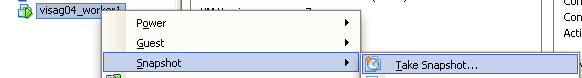
\includegraphics[width=0.5\textwidth]{./pic/snap_1.png}
	\label{fig:snap_1}
\end{figure}


Give a name to the snapshot (this name will be used in the virtual configuration of POP-C++), an optional description and click "Ok" (see Figure \ref{fig:snap_2}). 

\begin{figure}[ht]
	\caption{vSphere Client - Create Snapshot (Step 2)}
  	\centering
	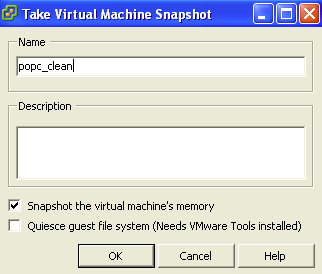
\includegraphics[width=0.5\textwidth]{./pic/snap_2.png}
	\label{fig:snap_2}
\end{figure}

The snapshot will be created (it can take a while to create the snapshot) and the worker will be ready to be used.

